\documentclass[12pt, oneside, a4paper]{abntex2}

% ---
% Pacotes básicos 
% ---
\usepackage{lmodern}			% Usa a fonte Latin Modern			
\usepackage[T1]{fontenc}		% Selecao de codigos de fonte.
\usepackage[utf8]{inputenc}		% Codificacao do documento (conversão automática dos acentos)
\usepackage{lastpage}			% Usado pela Ficha catalográfica
\usepackage{indentfirst}		% Indenta o primeiro parágrafo de cada seção.
\usepackage{color}				% Controle das cores
\usepackage{graphicx} 			% permite inserção de figuras
\usepackage{microtype} 			% para melhorias de justificação
\usepackage[alf]{abntex2cite}
\usepackage[a4paper,left=3.0cm,right=3.0cm,top=2.5cm,bottom=2.5cm]{geometry} 
\usepackage{setspace} 			% habilitando o espaço entre linhas
\usepackage{titlesec}
\usepackage[normalem]{ulem} 	% habilitando palavras sublinhadas
\usepackage{amssymb, amsmath, pxfonts} % permite símbolos matemáticos
\usepackage{mathrsfs} 			% permite uso de fontes para conjuntos
\usepackage{framed}
\usepackage{booktabs}
\usepackage{comment}
\usepackage[]{hyperref}
\usepackage{xr}
\usepackage[mathcal]{euler}
\usepackage{array}
\usepackage[brazil]{babel}
% ---

% ---
% Configurações UNIRIO
% ---
\linespread{1.3} 				% espaço entre linhas de 1.5
\setlength{\parskip}{10pt} 		% espaço entre parágrafos
\setcounter{secnumdepth}{3} 	% habilita a variável \thesubsubsection
\setcounter{tocdepth}{3} 		% Índice até subsubsection
\titleformat{\chapter}[hang]{\fontsize{16}{16}\normalfont\bfseries\filleft\selectfont}{\thechapter.}{0pt}{\normalfont\bfseries}
\titlespacing{\chapter}{0pt}{72pt}{60pt}
\titleformat{\section}[hang]{\fontsize{12}{12}\normalfont\bfseries\selectfont}{\thesection}{0pt}{\normalfont\bfseries}
\titlespacing{\section}{0pt}{24pt}{12pt}
\titleformat{\subsection}[hang]{\fontsize{12}{12}\normalfont\bfseries\selectfont}{\thesubsection}{0pt}{\normalfont\bfseries}
\titlespacing{\subsection}{0pt}{12pt}{6pt}
\titleformat{\subsubsection}[hang]{\fontsize{12}{12}\normalfont\bfseries\selectfont}{\thesubsubsection}{0pt}{\normalfont\bfseries}
\titlespacing{\subsubsection}{0pt}{6pt}{3pt}
% ---

\begin{document} 

 \pagestyle{empty}
        % Início da capa
\begin{figure}[!h]
    \centering
    
\includegraphics[scale=1.0]{imagens/unirio.png}
\end{figure}

\begin{center}
    UNIVERSIDADE FEDERAL DO ESTADO DO RIO DE JANEIRO \\ 
    CENTRO DE CIÊNCIAS EXATAS E TECNOLOGIA \\ 
    PROGRAMA DE PÓS-GRADUAÇÃO EM INFORMÁTICA
    \vskip 7.0cm

    Busca de Produtos Online com Base nas Necessidades dos Usuários
    
    
    \vskip 1.0cm

    Igor Veloso Custódio
    
    \vskip 2.0cm
    
\end{center}

\begin{flushright}
    \textbf{Orientador}

    Sean Wolfgand Matsui Siqueira
    
\end{flushright}

\vspace{\stretch{1}} % Posiciona o próximo texto no fim da página.

\begin{center}
    RIO DE JANEIRO, RJ - BRASIL \\ 
    Setembro de 2016
\end{center}
% Fim da capa
        % Início da folha de rosto
\begin{center}
    Busca de Produtos Online com Base nas Necessidades dos Usuários
    
    \vskip 1.5cm

    Igor Veloso Custódio
    \vskip 1.0cm

\end{center}

\begin{center}
DISSERTAÇÃO APRESENTADA COMO REQUISITO PARCIAL PARA OBTENÇÃO DO TÍTULO DE MESTRE PELO PROGRAMA DE PÓS-GRADUAÇÃO EM INFORMÁTICA DA UNIVERSIDADE FEDERAL DO ESTADO DO RIO DE JANEIRO (UNIRIO). APROVADA PELA COMISSÃO EXAMINADORA ABAIXO ASSINADA.
\vskip 1.0cm
\end{center}

\begin{flushleft}
    Aprovada por:
    \vskip 1.0cm

\end{flushleft}

\begin{flushright}
    \rule{10.0cm}{.1mm}

    Banca 1, D.Sc. - UNIRIO
    \vskip 0.5cm

    \rule{10.0cm}{.1mm}

    Sean Wolfgand Matsui Siqueira, D.Sc. - UNIRIO
    \vskip 0.5cm

    \rule{10.0cm}{.1mm}

    Banca 2, D.Sc. - UNIRIO
    \vskip 0.5cm

    \rule{10.0cm}{.1mm}

    Banca 3, D.Sc. - UFRJ
    \vskip 0.5cm
    
\end{flushright}
\vspace{\stretch{1}} % Posiciona o próximo texto no fim da página.
\begin{center}
    RIO DE JANEIRO, RJ - BRASIL \\ Setembro de 2016
\end{center}
% Fim da folha de rosto
        % Início da Ficha catalográfica
\vspace*{14.0cm}
\begin{framed}
    \fontsize{10pt}{10pt}\selectfont \hspace*{0.5cm} Oliveira, Andre Gustavo Ferreira de. \\ O48 \hspace{0.8cm}Busca de Produtos Online com Base nas Necessidades dos Usuários \\ \hspace*{1.3cm} Filosofia, Linguística e Psicologia / Andre Gustavo Ferreira de Oliveira, 2015. \\ \hspace*{1.3cm} 94f.; 30 cm.
    \vspace{0.3cm}

    \noindent \hspace*{1.5cm} \fontsize{10pt}{10pt}\selectfont Orientador: Leila Cristina Vasconcelos de Andrade \\ \hspace*{1.6cm} Coorientador: Sean Wolfgand Matsui Siqueira \\ \hspace*{1.6cm}Dissertação (Mestrado em Informática) - Universidade Federal do \\ \hspace*{1.2cm}Estado do Rio de Janeiro, Rio de Janeiro, 2015.
    \vspace{0.3cm}

    \noindent \hspace*{1.7cm} \fontsize{10pt}{10pt}\selectfont 1. Modelagem conceitual. 2. Programação orientada a objetos (Computação). 3. \\ \hspace*{1.5cm} Representação do conhecimento (Teoria da informação). I. Andrade, Leila Cristina \\ \hspace*{1.5cm} Vasconcelos de. II. Siqueira, Sean Wolfgand Matsui. III. Universidade Federal do \\ \hspace*{1.5cm} Estado do Rio de Janeiro. Centro de Ciências Exatas e Tecnologia. Curso de  Mestrado \\ \hspace*{1.5cm} em Informática. IV. Título.
    \vspace{0.3cm}
    \begin{flushright}
        \fontsize{10pt}{10pt}\selectfont CDD - 005.1
    \end{flushright}
\end{framed}
% Fim da Ficha catalográfica
 
 \pagestyle{empty}
 %\pagestyle{plain}
    %\pagenumbering{roman}
        % Início da Dedicatória
\vspace*{\stretch{1}} % Posiciona o próximo texto no fim da página.
\begin{flushright}
    As três mulheres da minha vida.\\
    A minha mãe por tudo que eu fui, eu sou e serei.\\
    A minha esposa, pel`O teu riso'.\\
    A minha filha, minha Victoria.\\
\end{flushright}
% Fim da dedicatóri
        % Início do Agradecimento
\begin{flushright}
    \vspace*{72pt}
    \fontsize{16}{16}\selectfont \textbf{Agradecimentos}
    \vspace{60pt}
\end{flushright}

\noindent
\hspace*{1.5cm}A minha mãe, por ser minha heroína! \\
\hspace*{1.5cm}A minha esposa, por sua dedicação, paciência e companheirismo nesse período tão conturbado, você foi minha fortaleza. \\
\hspace*{1.5cm}A minha orientadora, Professora Leila, pelo carinho e por me colocar nos trilhos. \\
\hspace*{1.5cm}Ao meu orientador, Professor Sean, pelas palavras certas, a paciência e a dedicação ao me guiar caverna afora. \\
\hspace*{1.5cm}Ao professor Bernardo, pelas palavras de incentivo e companheirismo. \\
\hspace*{1.5cm}Aos professores do PPGI, em especial a professora Fernanda e a professora Kate, pelos apontamentos e conselhos. \\
\hspace*{1.5cm}Aos amigos do SaL, por me ouvirem, ensinarem e colaborarem. Por compartilharem sorrisos e preocupações, todos são especiais. \\
\hspace*{1.5cm}Aos amigos da UFRRJ, pela compreensão, conselhos e participação. \\
\hspace*{1.5cm}Ao amigo Nilton, por todas as horas de conversas, todos os conselhos e por ser essa pessoa especial. \\
\hspace*{1.5cm}A Deus, por todas as vidas maravilhosas que tocam a minha.
% Fim do agradecimento
        % Início do resumo
Oliveira, Andre Gustavo Ferreira. \textbf{Um Processo de Modelagem Conceitual de Dados com Base em Teorias da Filosofia, Linguística e Psicologia.} UNIRIO, 2015. 94 páginas. Dissertação de Mestrado. Departamento de Informática Aplicada, UNIRIO.
\vspace{60pt}
\begin{center}
    \textbf{RESUMO}
    \vspace{60pt}
\end{center}

Modelagem Conceitual é definida como uma representação de um aspecto da realidade, onde as características relevantes para um contexto são evidenciadas para dar suporte a alguma atividade, em detrimento da complexidade inerente ao objeto real. O ato de modelar exige que o modelador, de maneira \textit{ad-hoc}, destaque as características de um objeto que são essenciais em um determinado contexto, porém essas características nem sempre se evidenciam com facilidade. Este trabalho propõe um processo que pretende guiar o modelador através de fases nas quais ele será capaz de entender a atividade que dá origem a um determinado conceito ao se deparar com um dado objeto. Por estar baseado nas teorias da Linguística, Filosofia e Psicologia, este processo pretende ajudá-lo a descobrir o melhor conceito possível para representar o conhecimento que o modelador quer expressar. O processo foi avaliado através de um estudo de caso, onde foram comparados modelos resultantes da sua utilização com modelos sem sua utilização. Nossos resultados sugerem que a utilização do processo auxilia modeladores a descobrirem: (1) como possuem o conhecimento acerca de um objeto, (2) quais características são importantes deste objeto que permitem a sua categorização e (3) como elas se relacionam, para dar origem ao conceito e, enfim, sua representação,Sistemas de Informação, Banco de Dados.

\vspace{20pt}

\textbf{Palavras-chave:} Modelagem Conceitual, Representação do Conhecimento, Conceitualização.
% Fim do resumo
        % Início do abstract
\begin{center}
    \textbf{ABSTRACT}
    \vspace{60pt}
\end{center}

Conceptual modelling is defined as a representation of an aspect of the reality, in which the relevant features for a context are evidenced to support some activity, to the detriment of the inherent complexity in the real object. The act of modeling requires that the modeler, in an ad hoc way, highlights the features of an object that are essentials in a certain context, however, not always these characteristics are evidenced with easiness. This master thesis proposes a process that intends to guide the modeler through phases in which he/she will be able to understand the activity that gives rise to a certain concept when faced with a specific object. As this process is based on the theories of the Linguistics, Philosophy and Psychology, it intends to help the modeler to discover the best possible concept to represent the knowledge that he/she wants to express. The process was evaluated through a case study whose models created using the process were compared with models that were created without using it. Our results suggest that the use of the process assists modelers to discover: (1) the knowledge concerning an object, (2) which characteristics are important of this object that allow categorizing it, (3) how they interact and give rise to the concept and, finally, its representation.

\vspace{20pt}

\textbf{Keywords:} Conceptual Modeling, Knowledge Representation, Conceptualization.
% Fim do abstract
        % Início do índice de texto
\tableofcontents
% Fim do índice de texto
         % Início do índice de figuras
\listoffigures
% Fim do índice de figuras
        % Início do índice de tabelas
\listoftables
% Fim do índice de tabelas
        %\include{pretexto/listaNomenclaturas}
 
 \pagestyle{headings}
    \pagenumbering{arabic}
    \setcounter{page}{1}
        \chapter{\hspace*{3pt} Introdução}

O homem desenvolve técnicas para representação de seu conhecimento, desde a antiguidade \cite{nonato:2009.teoria}. A comunicação, pouco a pouco, foi se tornando possível com o advento da fala, fazendo da oralidade a principal via de compartilhamento do conhecimento. A escrita, ainda em seus primórdios, tentava trazer esse conhecimento para uma esfera atemporal e, posteriormente, interespacial \cite{silva:2011.fala}. 

Com a expansão tecnológica, a partir do século XX, novas formas de representação do conhecimento surgiram, com objetivo de prover uma melhor maneira de capturar o mundo e seu conhecimento \cite{nonato:2009.teoria}. Diferentes autores, porém, ao longo dos séculos se ocuparam da tarefa de saber como se define o conhecimento, de como é possível ao homem conhecer e como o homem organiza esse conhecimento.

Com o surgimento da ciência cognitiva, na década de 60, pesquisas sobre cognição, natureza do conhecimento, funcionamento do cérebro e inteligência artificial, por exemplo, conseguiram avanços consideráveis, mostrando-se um campo promissor \cite{lacerda:2012.linguagem}.

\section{\hspace*{3pt} Justificativa}

A representação de conceitos não está isenta da subjetividade de quem o faz, nem do contexto na qual está inserida. Símbolos despertam em seus observadores conceitos que podem remeter a objetos distintos em contextos distintos \cite{nonato:2009.teoria}.

O ato de modelar é um trabalho que exige atenção e dedicação, para que os objetos percebidos sejam representados e despertem, nos observadores destas representações, os mesmos conceitos, ou ao menos conceitos mais próximos possíveis,que foram despertados naqueles que definiram essas representações.

Autores como \citeonline{vickery:1980.classificacao}; \citeonline{campos:2004.modelizacao} e \citeonline{alvarenga:2003.representacao} consideram as representações como essenciais às atividades humanas de registro e produção de conhecimento.

Um modelador precisa entender seu contexto, para ser capaz de criar uma representação que transmita sua exata percepção.  \citeonline{castro:2010.abordagem} aponta que um dos grandes problemas na modelagem conceitual é a dificuldade que o modelador possui de compreender os conceitos, e que sua experiência e o conhecimento que ele acumulou podem ser fatores preponderantes no processo.

As áreas da Linguística, Psicologia e Filosofia e suas teorias fortalecem o caráter multidisciplinar da área de Sistemas de Informação, além de oferecer um aporte teórico para a apreensão e entendimento dos objetos e conceitos que eles despertam \cite{lacerda:2012.linguagem}.

Desta forma esta pesquisa busca contribuir para o entendimento e representação destes objetos, o que justifica a necessidade de encontrar um processo que ajude a construção de modelos cuja representação possua qualidade semântica e pragmática, através da abordagem mista vinda de diferentes áreas do saber e de como lidam com a questão acerca do conhecimento.

\section{\hspace*{3pt} Objetivo Geral}

Analisar o processo de formação de conceitos e sua categorização, fundamentando em teorias da ciência cognitiva. Buscar compreender o processo desde a percepção do objeto até sua representação, e fornecer apoio para sua utilização no processo de descoberta de conceitos para modelagem conceitual.

\section{\hspace*{3pt} Objetivos Específicos}

Partindo da percepção, identificar as características essenciais de um conceito e como identificamos essas características e a maneira como elas se relacionam.
Classificar e Categorizar os conceitos, de acordo com sua relação contextual, permitindo que a cada nova agregação de características ou conceitos, novas relações sejam determinadas, permitindo a descoberta de novos conceitos.
Explicitar a formação dos conceitos em função de seus relacionamentos com outros objetos do contexto.
Propor um processo que possa guiar a descoberta de características e conceitos inerentes a um contexto.

\section{\hspace*{3pt} Metodologia}

Este trabalho utiliza um método de natureza aplicada, com objetivo descritivo, através de uma abordagem qualitativa. Para desenvolver a pesquisa, adotamos como modalidade o estudo de caso.

\section{\hspace*{3pt} Estruturação}

Este trabalho está dividido em seis capítulos. No capítulo 01 - Introdução, encontra-se a apresentação do tema da dissertação, a metodologia e a estrutura da dissertação. O capítulo 02 - Ciências Cognitivasapresentabrevemente os assuntos que tangem estadissertação e lhe servem de fundamentação teórica. Trata a questão da percepção, da categorização e da formulação dos conceitos efetuada pelas áreas da Filosofia, Psicologia eda Linguística. O capítulo 03 - Modelagem Conceitual trata da questão da representação do conhecimento, em especial através da abordagem de Modelos Conceituais. Neste capítulo também é descrito um estudo preliminar a fim de entender como se dá o processo através do qual os modeladores entendem e representam um contexto. No capítulo 04 - POR: Processo Objeto-Representaçãoapresentamos nossa proposta e o fluxo resultante do processo. No capítulo 05 - Avaliaçãodescrevemos as avaliações do processoe, finalmente, no capítulo 06 - Conclusões são apresentadas algumas observações sobre o trabalho, bem como sugestões para trabalhos futuros.
        \chapter{\hspace*{3pt} Ciências Cognitivas}

Neste capítulo vamos discorrer de maneira breve sobre as principais áreas que discutem a possibilidade de aquisição do conhecimento pelo homem, assim como a sua representação.

Dado este propósito, parece impossível não tanger a área das ciências cognitivas, área interdisciplinar que, segundo \citeonline{lacerda:2012.linguagem}:
\begin{quote}
[...]descreve, explica, e, eventualmente, simula as principais disposições e capacidades da cognição humana: a linguagem, a percepção, a coordenação motora e a planificação, objetivando entender a aquisição de conhecimentos ou das percepções dos seres humanos e de seus processos mentais \cite{lacerda:2012.linguagem}.
\end{quote}
\apudonline{casti:1989.paradigms}{saracevic:2008.ciencia} define Ciência Cognitiva como a ``[...] amálgama de psicologia, filosofia, antropologia, neurofisiologia, ciência da computação e linguística, organizada em torno do uso do computador enquanto ferramenta capaz de extrair os segredos da mente”.

O hexágono cognitivo, Figura 1, mostra como se daria o relacionamento entre essas áreas, destacando a natureza de seu vínculo, isto é, as disciplinas que possuem um forte vínculo interdisciplinar, representado pelas linhas fortes, e as que possuem vínculo interdisciplinar fraco, representado pelas linhas tracejadas \cite{lacerda:2012.linguagem}.

\begin{figure}
    \centering
    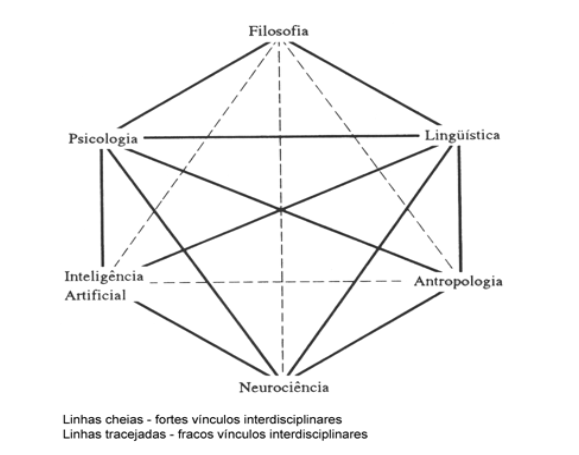
\includegraphics[width=\textwidth]{imagens/hexagono_cognitivo.png}
    \caption{Relações entre as Ciências Cognitivas. Fonte: \apudonline{gardner:1995.nova}{lima:2003.interfaces}}
    \label{fig:hexagono_cognitivo}
\end{figure}

Neste trabalho, por uma questão de redução de escopo, nos ocuparemos principalmente pelo seu forte vínculo interdisciplinar e discurso associativo com o tema proposto para investigação, das áreas da Filosofia, Psicologia e Linguística, através das teorias que dão fundamentação a esta dissertação.

\section{\hspace*{3pt} Conhecimento}

Com o advento da escrita, e até antes disto, com as representações pictográficas, ao homem foi possível romper as limitações de sua própria existência para a preservação do conhecimento. A representação do conhecimento, é desta maneira, o ponto determinante do processo informacional, visto que recai sobre ela a tarefa de manifestar o saber sobre seres e as coisas do mundo real para aquele que será o usuário final da informação \cite{caixeta:2008.representacao}.

Tão importante quanto sua representação, o que podemos definir como sendo conhecimento, e o que possibilita ao homem adquiri-lo desperta a atenção dos estudiosos, desde a Grécia antiga.

De maneira bem ampla, podemos definir conhecimento como a relação entre o sujeito e o objeto, onde a função do sujeito é apreender o objeto e a função do objeto é ser apreensível e ser apreendido pelo sujeito, com a finalidade de dominá-lo e utilizá-lo para entendimento e elucidação da realidade.

As questões acerca da possibilidade de conhecer, no entanto, apresentam diferentes correntes e teorias. No campo da Filosofia, o criticismo propõe que o conhecimento só é possível devido a sensibilidade que dá à matéria do saber e ao entendimento, que dá às formas do conhecimento, sendo esta uma teoria intermediária entre a teoria empirista e a teoria racionalistas \cite{kant:1983.critica}.

A sensibilidade nos fornece intuições, representações singulares que se referem imediatamente aos objetos particulares, e o entendimento produz conceitos, representações gerais que se referem sempre a outras representações(imediatamente aos objetos) \cite{pereira:2011.espaco}.

Geralmente o vocábulo conceito é usado para referir-se a uma unidade do conhecimento (Gercina Ângela Borém Lima, 2007). Segundo o dicionário online Priberam, (2015), o termo “conceito” tem origem na palavra latina “conceptus” (do verbo concipere) que pode ser traduzida como “coisa concebida” ou “formada na mente”, e pode significar, entre outros: 1. Concepção compreendida numa palavra que designa características e qualidades de uma classe de objetos, abstratos ou concretos; 2. Opinião ou ideia, juízo que se faz de alguém ou de alguma coisa; 3. Expressão sintética.

Conceito é uma noção abstrata, uma representação mental referenciada em cada palavra de uma língua que corresponde a um conjunto de propriedades comuns a um grupo de seres - reais ou abstratos - ou objetos, determinando como as coisas são.

De acordo com Paul Thagard; Ethan Toombs, (2005), essas representações mentais, geralmente, correspondem e se referem a classes de coisas do mundo.

2.2. Linguística

Dahlberg preocupada com a compreensão da importância do conceito, na representação do conhecimento, explicita o estudo sobre conceitos na Ciência da Informação (Nonatto, Rafael dos Santos, 2009). A teoria do conceito busca uma base mais sólida para determinar e entender o que consideramos como um conceito (Campos, Maria Luiza de Almeida, 2001).

A autora apresenta ainda o triângulo semântico de Ogden e Richards (Ogden, Charles Kay et al., 1923), Figura 2, que serve como modelo para construção de conceitos, e onde estão representadas as relações entre o objeto ou o referente, o conceito ou o pensamento/referência e o termo ou símbolo.


Triângulo Semiótico.

Sabemos que o homem tem a capacidade de fazer afirmações sobre as coisas reais e sobre ideias que existem apenas em sua mente, através das linguagens naturais, linguagens utilizadas nas necessidades da vida cotidiana (Campos, Maria Luiza de Almeida, 2001).

Essas afirmações, ou enunciados, podem falar a respeito de objetos da sensibilidade ou de objetos do entendimento, de maneira geral ou de maneira individuais. Os objetos gerais são aqueles que estão situados fora de um espaço e um tempo específico, um contexto, e constituem-se de enunciados mais genéricos. Os objetos individuais, por outro lado, podem ser pensados como exclusivos e distintos dos demais, isto é, constituem uma unidade inconfundível. Por exemplo, podemos falar sobre Clint Eastwood ou sobre atores do cinema Western, para exemplificar conceitos específicos ou gerais, respectivamente (Dahlberg, Ingetraut, 1978; Dahlberg, Ingetraut, 1978).

Na teoria proposta por Dahlberg, as características desempenham um papel fundamental. Ela define um conceito como uma série de enunciados, isto é, características verdadeiras sobre um objeto, reunidos de maneira sintética, sob uma ``tag'', um signo capaz de representar essa síntese.

Dahlberg também faz uma distinção importante entre unidade do pensamento e unidade de conhecimento. Segundo ela, a unidade de pensamentotransmite uma ideia de subjetividade enquanto a unidade de conhecimentoremete a um entendimento objetivo. A figura 3, representa os três passos envolvidos na formação de um conceito (Campos, Maria Luiza de Almeida, 2001).


Modelo para Construção de Conceitos em Dahlberg.
No momento em que selecionamos um objeto, tem-se início o processo de determinação de um conceito. Atribuímos predicados a este objeto, destacando as suas características mais relevantes. ParaIngetraut Dahlberg, (1978), as características relevantes são aquelas necessárias para queo objetoseja exatamente ele e não outro. Essas característicasauxiliam o processo de designação do objeto, e a junção destas característicasdevem ser expressas ou representadas por um signo.

Nossa comunicação, designando os objetos que estão ao nosso redor e transmitindo os pensamentos, que somos capazes de formular em nossos íntimos, sobre esses mesmos objetos só nos é possível graças à linguagem; a princípio um conjunto de símbolos pictográficos, que ganharam regras e representações sonoras, originando a fala e a escrita (Dahlberg, Ingetraut, 1978).

Desde a nossa infância, fomos habituados aassociar os objetos asons e sinais pré-determinados. Tornando-se natural, no decorrer de nossas vidas, que nossa percepção trabalhe com representações icônicas (figuras e imagens), um mundo visual que está ao nosso redor(Engelkamp, J., 1976)apud(Dahlberg, Ingetraut, 1978). REVER

2.3. Filosofia

A preocupação em nomear, definir e categorizar as coisas do mundo é antiga e passou de um processo individual a um processo cultural e social. Lima, Gercina Ângela Borém, (2007), em consonância com outros autores, considera os termos categorização e classificação como sinônimos.

Categorização ou classificação é o processo cognitivo de dividir as experiências do mundo em grupos de entidades ou categorias, para construir uma ordem física e social do mundo (Lima, Gercina Ângela Borém, 2003). Na concepção dada por Iyer, Hemalata, (1995), as categorias concedem estabilidade e ordem ao mundo que percebemos, segmentando-o, possibilitando agrupamentos de objetos de formas utilizáveis, nesse sentido, torna-se impossível pensar sem formar categorias (Artêncio, Luciane Maria, 2012).

A categorização, segundo Silva, Alessandra Rodrigues da; Lima, Gercina Ângela Borém, (2011), é o processo cognitivo de compreensão das características dos objetos por critérios de similitude ou diferença. Entretanto, Artêncio, Luciane Maria, (2012)argumenta que atualmente a categorização não vem recebendo a atenção que lhe é necessária nos estudos desenvolvidos na Ciência da Informação:

Ainda que contemporaneamente a categorização seja assumida, ou como parte da capacidade intelectual necessária ao ser humano para a efetivação do processo cognitivo, ou como expressão sócio-cultural de organizar o mundo, de um modo geral, ela não tem sido reconhecida como uma questão presente nos discursos da Ciência da Informação (Artêncio, Luciane Maria, 2012).
Aranalde, Michel Maya, (2009),em um tratamento contemporâneo e com respaldo da filosofia e da teoria da classificação, defende:

As categorias são identificadas como conceitos elementares, isto é, como princípios que permitem identificar as notas essenciais que caracterizam um objeto de conhecimento. A partir desta operação mental de identificação, é possível formular conceitos empíricos, ou seja, buscar uma equivalência entre como o objeto se apresenta e a representação mental que se faz dele e de suas relações com outros objetos. As categorias são concebidas como meta-conceitos que permitem a efetiva conceitualização de objetos passíveis de serem conhecidos, organizados e classificados. Portanto, elas são elementos intermediários entre os conceitos e a realidade cognoscível(Aranalde, Michel Maya, 2009).
Blair, David, (2006) concebe as categorias como a base da linguagem. A categorização, sob sua perspectiva, é uma forma de simplificação que provê um sistema de referência básico no qual coisas que são fundamentalmente diferentes são tratadas como se fossem semelhantes(Artêncio, Luciane Maria, 2012).

A capacidade de listar as características do objeto percebido e compará-las a de outros objetos já conhecidos, é um privilégio da racionalidade humana, que permitem a percepção, classificação e criação de conhecimentos acerca dos objetos(Alvarenga, Lídia, 2003).

A organização do conhecimento, da sua representação à sua recuperação, está estritamente relacionada com os conceitos que compõemo campo do saber abordado e as relações entre eles, tendo em mente a influência do contexto, em qualquer descrição e representação individual dos mesmos(Lima, Gercina Ângela Borém, 2003).

Corroborando com esta ideia,Mauss, Marcel, (1999) , explica que existe um relação estreita entre os sistemas sociais e suas relações lógicas, reforçando a ideia de que em torno de um signo, em sua representação ampla, existe a participação coletiva e social, fruto de um arranjo semântico de uma comunidade, de uma raça, de uma sociedade(Artêncio, Luciane Maria, 2012).

Com a linguística, a categorização passou a ser encarada por outro viés, se ocupar dos métodos utilizados pelos sujeitos para categorizar, descrever, justificar, compreender os fenômenos da vida cotidiana(Jan Edson Rodrigues-Leite, 2005).

2.4. Psicologia

A psicologia, apresenta algumas teorias para a construção do conhecimento. Piaget, por exemplo, defende que a representação funciona através de signos, que durante a construção do conhecimento são associados a imagens mentais, o que permite sua evocação posterior, em outro objeto ou atividade(Smolka, Ana Luiza B, 1993).

O modelo de protótipo, defende que conceitos são representados por um grupo de características, e não por suas definições. O agrupamento de conceitos em uma dada categoria se daria, segundoRosch, Eleanor, (1999), não pela alternância dos traços dicotômicos, mas pela semelhança com o protótipo, em que um membro condensasse os traços mais característicos da categoria.

O pilar desta teoria, sustenta que as categorias são organizadas em torno de protótipos centrais, isto é, um exemplo representativo de uma categoria seria aquele que compartilhasse com os outros membros de sua categoria o maior número de características e que, por outro lado, compartilhasse de poucas características, ou nenhuma, com elementos de fora desta(Lima, Gercina Ângela Borém, 2007).

Rosch, Eleanor, (1999), propõe uma série de experimentos onde comprova que existem dois princípios gerais e básicos para formação de categorias. O primeiro afirma que a tarefa dos sistemas de categoria é fornecer o máximo de informação com o menor esforço cognitivo, princípio que ela denomina como economia cognitiva (tradução livre de Cognitive Economy); o segundo afirma que o mundo percebido se apresenta através de informações estruturadas em vez de atributos arbitrários ou imprevisíveis, princípio nomeado de estrutura do mundo percebido (tradução livre de Perceived World Structure).

Esses dois princípios, combinados, implicam para o nível de abstração de categorias formadas em uma cultura e para a estrutura interna das categorias, se apresentando em duas dimensões: a vertical e a horizontal (Rosch, Eleanor, 1999).

A dimensão verticalintroduz o conceito de objetos de nível básico, diz respeito a capacidade de inclusão de uma categoria, isto é, qual categoria é mais abrangente e qual é menos. A dimensão horizontal diz respeito à segmentação de categorias no mesmo nível de inclusividade. Como uma categoria se organiza internamente, ou seja, temos categorias distintas, dentro do mesmo grau de inclusão. A Figura 4demonstra níveis de categorização nas duas dimensões e apresenta alguns exemplos (Lacerda, Naziozenio Antonio, 2012).

Níveis de Categorização
Como podemos ver, as dimensões demonstram que o nível básicoé o nível mais equilibrado, ou seja, é o nível onde os conceitos são mais expressivos e há uma maior economia cognitiva, isto é, um resumo dos atributos importantes que distinguem uma categoria da outra.

        \chapter{\hspace*{3pt} Modelo Conceitual}
\label{chap:modeloConceitual}

Modelo é a representação abstrata e simplificada de um sistema real, com a qual se pode explicar ou testar o seu comportamento em seu todo ou em partes \cite{cougo:1997.modelagem,castro:2010.abordagem}.

Dada a complexidade do mundo em sua totalidade a e necessidade do homem em entender a realidade, os modelos possuem a função de simplificar a realidade de maneira inteligível, permitindo ao homem apreendê-lo e compreendê-lo em suas partes essenciais para um determinado domínio ou campo de estudo (Almeida, Maurício Barcellos, 2006; Dodebei, Vera, 2002).

O processo de modelar demanda o deslocamento do mundo dos fenômenos para um espaço de representação. Modelar o mundo e representar o conhecimento disponível requer entendimento dos papéis que tal representação pode desempenhar campos \cite{campos:2004.modelizacao}.

Os modelos são entidades importantes e integram as raízes do método científico: “[...] todas as teorias e modelos científicos são aproximações da verdadeira natureza das coisas; o erro envolvido na aproximação é não raro, suficientemente pequeno para tornar significativa essa aproximação” \apud{capra:1983.tao}{almeida:2006.modelo}.

Os modelos conceituais têm por objetivo desenvolver uma descrição coerente do significado dos dados, satisfazendo nossas necessidades de conhecimento e conceituação sobre determinado domínio, antecipando ou substituindo a existência de uma realidade qualquer \cite{higuchi:2012.representaccao}.

Os modelos devem, portanto, servir como fontes de referência, quando dúvidas acerca do domínio surgirem, e como um repositório de conhecimento comum, auxiliando a comunicação, o aprendizado e o seu reuso em um nível mais alto de abstração \apud{arango:1994.domain}{guizzardi:2000.desenvolvimento}.

A perspectiva cognitiva é adotada por vários modelos na Ciência da Informação: modelos de representação de usuários e suas necessidades, modelos de representação de estratégia de busca, modelos de representação de documentos. Os primeiros modelam situações problemáticas dos usuários frente a sistemas de informação; os segundos examinam os aspectos cognitivos do processo de transferência de informação entre o usuário e o especialista da informação; e os últimos podem ser modelos mentais do usuário, segundo a perspectiva do sistema, ou modelos conceituais apresentados ao usuário pelo projetista do sistema \cite{sayao:2001.modelos}{almeida:2006.modelo}

Metamodelos distintos são utilizados para a representação de Modelos Conceituais, porém o processo de modelagem é anterior a sua representação. Com o intuito de entender como modeladores distintos, reagem a tarefa de representar, através de um modelo, o seu entendimento acerca de um domínio e como o ato de modelar desperta suas próprias experiências para que possam expressar os conceitos, realizamos um estudo de caso.

3.1. Primeiros Estudos

Para esse estudo, foram convidados cinco analistas de sistemas de informação, com experiência, acadêmica ou profissional, na elaboração de modelos conceituais. O perfil foi definido buscando casos que pudessem exemplificar entre analistas os extremos entre suas experiências \cite
(Wainer, Jacques, 2007).

Nossa questão norteadora foi a de saber como diferentes pessoas interpretam um contexto e como suas experiências pessoais podem se refletir sobre sua representação acerca desse mesmo contexto?

Os dados foram coletados através da gravação do processo de modelagem e os participantes passaram por uma entrevista ao final do processo.

Como tarefa, os participantes deveriam analisar o contexto de uma rede de cinemase baseados em suas experiências e conhecimentos sobre a área de negócios e atuação de cinemas em geral, construir um modelo que fosse capaz de representar seu conhecimento sobre as atividades deste contexto e suas relações existentes. Foi sugerido que os participantes considerassem toda atividade ou processos que julgassem pertinentes ao contexto e, se possível, vislumbrassem a expansão do negócio (novas salas, novos cinemas, vendas on-line, tudo que julgassem necessário de acordo com sua experiência).

Para a representação do modelo, o participante poderia utilizar a linguagem que ele se sentisse mais àvontade ou tivesse maior domínio (ER, UML, OntoUML, OWL, etc.)

Sobre o domínio, todos os participantes relataram nunca terem precisado criar quaisquer tipos de modelos ou descrições explícitas sobre o contexto, embora tenham o hábito de frequentar cinemas ao menos uma vez ao mês, em média. Isso lhes garantiu, segundo a maioria dos relatos, uma visão superficial do contexto. Um dos participantes ressaltou que a correta representação de um domíniodepende doaprofundamento de estudos acerca de seu funcionamento.

Embora tenham alegado um conhecimento parco acerca do domínio, quando indagados, nenhum deles relatou quaisquer problemas para efetuar o modelo. O que sugere que as características dominadas e consolidadas como unidade de conhecimentopermitiram gerar conceitos determinados e falar sobre o contexto com propriedade, de acordo com suas experiências e vivências.

Um ponto a destacar, diz respeito a suas concepções acerca do domínio. Apesar de nenhum relatar dificuldade, a apresentação da tarefa, propositalmente, descrevia o domínio com um conceito geral: "cinema. A ideia era despertar a maior quantidade de conceitos subalternos possíveis que os participantes fossem capazes de acessar. Porém todos sentiram a necessidade de questionar quais abordagens deveriam seguir para suas representações.

Neste aspecto, podemos perceber que a contextualização está fortemente associada a maneira como definimos nossos conceitos. Na falta de umcontexto explícito, todos optaram por seguir a contextualização do usuário, isto é, representar o seu próprio entendimento, os aspectos que estavam acostumados a interagir e da maneira como o faziam.

A experiência pessoal, neste sentido, foi bastante importante. Embora todos reconheçam de alguma maneira que é preciso fazer a compra do ingresso, descrever esse processo através do modelo trouxe dificuldades. Alguns participantes, relataram que pensar sobre essa questão exigiu uma maior dedicação, em parte por possuírem regras que não dominavam e em partepor agregarem novos conceitos ao contexto, como por exemplo: o processo de compra on-line.

Os participantes que já haviam, de alguma maneira, lidado com questões semelhantes, conseguiram representar essa tarefa traçando um paralelo entre tarefas ou mesmo domínios semelhantes. Destacamos aqui aqueles com maior tempo de atuação no mercado de trabalho.

A formação acadêmica dos participantes não foi um fator que representasse desvio na análise, visto que se mostrou bastante homogênea, apenas um dos entrevistados havia feito ensino médiocom formação técnica, e todos possuíam ou estavam na pós-graduação, além de possuírem domínio acerca do metamodelo UML, ou outro equivalente, e já terem trabalhado com bancos de dados, ao menos em algum grau. Convém ressaltar que a utilização da UML, como forma de representar o domínio, não foi uma escolha unânime.

3.2. Descrições dos Processos para Modelagem

Descreveremos de maneira mais detalhada possível, como se sucedeu a execução das tarefas por cada um dos participantes, de maneira a tentar demonstrar, passo a passo, como exteriorizaram o seu conhecimento acerca do domínio. Em alguns casos, foi possível perceber que alguns símbolosderam lugar a outros, conforme a modelagem avançava, em outros casos, que após a inserção de um determinado símbolo, outros conceitos eram alcançados, em seguida.

3.2.1. Participante 001

Ao iniciar a tarefa,o participante utilizou o MySQL Workbench para lhe auxiliar, optando por uma linguagem UML para representar seu modelo conceitual. Ao ser apresentado à tarefa, o participante questionou que tipo de visão deveria priorizar, ao que foi respondido que deveria seguir sua própria experiência e interações com o contexto.

O participante adotou uma abordagem top-down, partindo de agrupamentos mais amplos, nomeados com conceitos gerais e pouco a pouco adicionando os conceitos mais específicos. Pôde-se observar que o participante possui um forte senso de organização, preocupando-se em criar previamente, com a ferramenta adotada, espaços - denominados layersna ferramenta - que representavam os conceitos gerais e que iriam servir como agrupadores para os conceitos mais específicos.

Por ser o contextouma rede de cinemas, o participante 001 entendeu que o conceito principal deste era FILME, sendo esta a primeira entidade adicionada ao seu modelo. O participante rapidamente identificou três características relacionadas ao conceito filme: id, nomee categoria. Por estar utilizando uma abordagem de banco de dados, a teoria sugere que para evitar duplicidade de informação na armazenagem de dados, todo dado deve ter um identificador único (Heuser, Carlos Alberto, 2001; Machado, Felipe Nery Rodrigues; Abreu, Maurício Pereira de, 2009); que foi representado nesta modelagem como id, sendo então adicionado como uma característica ao conceito de filme, assim como nome. O conceito de nome, sendo adicionado como propriedade de filme, sugere uma intensão específica, na qual um nome está associado única e exclusivamente a um filme, embora o conceito nome possa ter extensão ao se referir ao grupo de todos os nomes possíveis atribuídos a objetos e indivíduos (Dahlberg, Ingetraut, 1978). Por fim, o participante entendeu que o conceito CATEGORIA, embora fosse uma propriedade de filmes, consistia em uma relação na qual uma mesma categoria de filmes poderia estar associada a diferentes filmes, gerando por esse motivo uma nova entidade. Como propriedades dessa entidade, foram encontrados ide nome.

O participante nomeou o layerque continha essas duas entidades como FILMES, entendendo que FILME é um agrupamento categorial que engloba os conceitos de Filmes e Categorias.

Dando prosseguimento em sua modelagem, o participante nomeou o segundo layercomo CINEMA, sugerindo que todos os conceitos que fizerem parte desse agrupamento categorial serão inseridos neste espaço. Para esse layer, encontrou de imediato o conceito SALAS, cujas propriedades identificadas foram: id, nomee lotacao.

O terceiro layerfoi considerado o agrupamento categorial de todos os conceitos envolvidos com vendas e por esse motivo, o participante o nomeou como PDV (Ponto de Venda).

O primeiro conceito encontrado nesse agrupamento foi o de VENDAS. Essa entidade continha como características os conceitos de ide produto. Sendo produto, um conceito que substituiu seus análogos nas outras tabelas, conhecidos como nome. Produto sugere a existência de um agrupamento intermediário entre vendas e nome, um conjunto formado por outros conceitos, ainda não analisados, cujo conceito nome está contido.

O segundo conceito pertencente a esse agrupamento categorial, foi de INGRESSO, sugerindo que o participante faz uma distinção entre os tipos de compras que se pode fazer em um cinema. Como propriedade, foram encontrados ide filme, sendo este último imediatamente substituído por produto, e por fim, por venda. Sugerindo que esse conceito se relaciona com o conceito de venda, pertencendo a este, mas sendo importante para o contexto a ponto de estar em uma tabela a parte.

No quarto layer, chamado de marktplace, o último dos quatros criados inicialmente, foi inserido o conceito de HORARIOS, cujas propriedades adicionadas foram id, filme, sala, horario, onde, filme se relaciona com o conceito FILME, através da relação horario-filme. Sala se relaciona com o conceito SALAS, através da relação horario-sala.

Outro conceito adicionado a essa agrupamento foi o de PRODUTO. Observou-se que o participante demorou aproximadamente 25 segundos decidindo se esse conceito deveria pertencer ou não ao agrupamento, e a identificação de suas propriedadespareceram gerar hesitação. Por fim, as propriedades adicionadas foram: id, horarioe valor. A relação entre PRODUTOe HORARIOS, pareceu gerar igualmente indecisão, mas no fim, o participante optou por adicionar a relação produto-horario. Na sequência, a relação entre os conceitos PRODUTOe VENDAfora estabelecida pela relação venda-produto.

A relação entre INGRESSO e VENDA, denominada ingresso-venda, apresentou demora quanto sua decisão de inserção.

A partir deste ponto, o participante pareceu procurar de maneira mais cuidadosa propriedades e relações que pudessem fazer parte dessa representação. Novos conceitos, fossem com grande extensão ou intensão, não pareceram estar mais tão evidentes ao participante quanto os primeiros.

Uma análise mais cuidadosa dos conceitos já inseridos e em suas relaçõesrevelou mais duas propriedades, para o conceito VENDA, a saber: identificadore status emais uma propriedade para o conceito INGRESSO, identificador.

Após mais alguns segundos analisando o fluxo possível para execução do processo de compra de ingressos e produtos, o participante julgou necessária a presença de um novo conceito no agrupamento PDV. Esse conceito foi identificado como OPERADOR, e lhe foram atribuídas as seguintes propriedades: ide funcionario. No primeiro momento, funcionário foi definido de forma que sugeria a futura inserção de um conceito FUNCIONARIO que teria relação com o conceito operador, novamente trazendo a ideia de hierarquização entre os conceitos, onde o conceito operador estaria incluído no conceito funcionário.

A presença do conceito OPERADORse refletiu na necessidade de edição do conceito VENDAS, para a inserção de uma nova relação, denominada venda-operador. No agrupamento cinema, o participante adicionou o conceito PESSOA, optando por um conceito geral para sua representação, lhe atribuindo as propriedades idenome. A partir deste conceito com extensão geral, traçou a relação com o conceito OPERADOR, nomeando como operador-pessoa.

Somente após 8 minutos de observação, o participante adicionou uma nova propriedade ao conceito PRODUTOcadeira e um novo conceito, desta vez um sendo originado pela ideia de relação entre venda-produto. Esse conceito originou a tabela homônima, cujas propriedades definidas foram: id, vendae produto. Esse conceito mantém, como o nome sugere, relação com o conceito VENDA, através da relação venda e com o conceito PRODUTO, através da relação produto. Desta forma, o participante descartou a relaçãovenda-produtopreviamente estabelecida.

No conceito INGRESSO, a propriedade utilizada foi acrescida, sugerindo a ideia de que um ingresso pode ou não ter sido utilizado, após sua aquisição e finalizando o modelo do usuário, que utilizou mais 6 minutos para alguns ajustes de apresentação e organização, totalizando aproximadamente 40 minutos para execução da tarefa.

A Figura 5representa o modelo gerado pelo pelo participante 001 ao término da tarefa.


Modelo gerado pelo participante 001.
3.2.2. Participante 002

O participante 002, ao ser apresentado ao contexto e a tarefa de representá-lo, pontuou algumas dúvidas acerca desta. O contexto, embora definisse o domínio, carecia de uma visão mais focada que guiasse o participante na direção de uma representação mais específica. Outra dúvida fora sobre a maneira que ele poderia representar o contexto, isto é, que ferramentas ou linguagens poderia se valer para a execução da tarefa.

Fora explicado ao participante que o mesmo deveria tomar as circunstâncias que lhe fossem mais comuns para a representação do contexto e poderia se valer de qualquer linguagem que lhe parecesse mais simples ou detivesse maior experiência de uso. Tendo esclarecido estas questões, o participante optou por utilizar a linguagem E-R, disponibilizada em uma ferramenta web para executar seu modelo.

Seguindo as orientações, o participante definiu primeiro todas as entidades que ele julgou pertinentes ao contexto na seguinte ordem: GRUPO, FILIAL, SALA, LOCALIZACAO, SERVICO, FUNCIONARIO, FILME, SESSAO e DISTRIBUIDORA.

Sua abordagem seguiu a visão \textit{top-down}, onde a entidade mais geral, o grupo que representa todas as salas de cinema, foi a primeira a ser definida, e cada conceito pertencente ao primeiro, fora definido um após o outro.

Após determinar todas as entidades, o participante 002 representou cada uma das relações que as entidades possuíam umas com as outras, de acordo com a sequência: GRUPO se relaciona com FILIAL, FILIAL com FUNCIONARIO e com SALA, SALA por sua vez se relaciona com SESSAO e LOCALIZACAO. Neste ponto, o participante ficou confuso quanto ao tipo de relacionamento que SALA manteria com LOCALIZACAO. Dando continuidade aos relacionamentos, o participante 002 definiu a relação entre SESSAO e FILME, FILME com DISTRIBUIDORA e LOCALIZACAO com SERVICO.

O participante 002 precisou definir ainda as seguintes entidades INGRESSO, CANAL DE VENDA e CONTRATO, traçando a relação de SESSAO com INGRESSO, INGRESSO com CANAL DE VENDA, GRUPO com CONTRATO, CONTRATO com DISTRIBUIDORA.

Neste ponto, mais uma entidade precisou ser definida, USUARIO ON LINE, que foi relacionada com INGRESSO, gerando novamente dúvidas sobre o tipo de relacionamento que manteriam uma com a outra.

Como última etapa do processo de modelagem, o participante 002 definiu as características de cada entidade da seguinte maneira:

GRUPO(sede,marca,empresa,cnpj); CONTRATO(valor, vigencia, logistica); FILIAL(cnpj, responsavel); FUNCIONARIO(nome, cpf, salario, funcao, cargo); LOCALIZACAO( shopping, endereço);SALA(mapa de cadeiras, código,3d,imax, conforto premium); DISTRIBUIDORA(responsavel,cnpj, contato);FILME(titulo, classificacao, descricao, midia, trailer);SESSAO(horario, dublado/legendado,3D); SERVICO(pipoca, promocoes,bebida, doces, valor); INGRESSO(beneficio meia?, valor inteira, data compra, forma de pagamento*); CANAL DE VENDA(internet, guiche); USUARIO ON LINE(id, nome).

Pode se observar, porém, que na entidade GRUPO, o participante teve dúvidas acerca de que símbolo utilizar para representar o conceito do nome do grupo da empresa. A palavra riscada, representa o signo preterido em favor do signo escolhido, marca. A características forma de pagamento, marcada com asterisco (*), somente foi acrescentada após as definições das características de Canal de Venda, evidenciando que um conceito conectou ao outro.

A preocupação do participante 002 em demonstrar informações como distribuidora, classificação, tipo de mídia, se a cópia é dublada ou legendada, por exemplo. Isso pode significar uma maior experiência em relação ao contexto apresentado e sua atividade fim. Seu tempo total de execução do modelo foi de aproximadamente 20 minutos.

A Figura 6, representa o modelo gerado pelo pelo participante 002 ao término da tarefa.


Modelo gerado pelo participante 002.
3.2.3. Participante 003

O participante 003também ficou em dúvidas ao ser apresentado à tarefa, questionando como, exatamente, deveria efetuar o modelo. Ao qual foi esclarecido, que assim como constava nas orientações, ele deveria escolher o método para representação que se sentisse mais a vontade e que melhor demonstrasse as particularidades do contexto. Quando questionou sobre que tipo de informações deveria priorizar no modelo, lhe foi solicitado que representasse aquelas que ele julgasse necessárias para demonstrar seu conhecimento sobre a mesma, de maneira clara.

O participante 003 optou por executar a tarefa através de uma descrição textual das entidades, relacionamentos e propriedades. A primeira entidade descrita por ele, foi FILME, com os atributos básicos títuloe duração. Pode-se perceber aqui a associação do conceito cinema, representando o contexto, ao conceito filme, como um conceito mais específico, conforme apresentado por (Dahlberg, Ingetraut, 1978). A próxima entidade descrita foi SALA, com o atributo nome. E depois a entidade CLIENTE, e seus atributos: nomee endereço, sendo essa última como uma referência para a entidade, ainda vindoura. A próxima entidade descrita fora FUNCIONÁRIO, possuindo também os atributos nomee endereço, endereço também como referência.

A entidade CINEMA, foi a quarta entidade a ser descrita e continha os atributos nome, salase endereço. O símbolo escolhido para representar o conceito sala, estava na forma plural, demonstrando que o participante entende que o conceito cinema, por ser geral, pode conter mais de uma sala, mas apenas um endereço, por esse motivo a falta da forma plural deste último signo. Outro indicador de que as noções hierárquicas estão presentes na modelagem, é o fato que ambos os atributos, entraram como referências a outras entidades.

A entidade SESSÃO, com os atributos horário início, horário fim, preço, número total de assentos, funcionário responsável, comreferência àentidade FUNCIONÁRIO,foi definida. Ainda durante a definição do conceito FUNCIONÁRIO, o participante 003 adicionou o símbolo número, aos símbolos total de assentos, que representavam essa característica.

COMPRA, com os atributos cliente,sessão, número do assento compradoe forma de pagamento, foram definidos. o atributo cliente fazendo referência para a entidade CLIENTEe o atributo sessão, fazendo referência para a entidade SESSÃO.

A entidade AVALIAÇÃOcom os atributos comprafazendo referência àentidade COMPRAe o atributo nota da avaliaçãoforam descritos logo após.

O participante julgou ser preciso esclarecer a necessidade de elaboração de regras para o melhor entendimento do modelo, com por exemplo verificar a quantidade de assentos disponíveis e se um determinado filme "caberia"em uma sessão.

Ao analisar os conceitos definidos, recordou-se que embora prevista, ainda não havia definido a entidade ENDEREÇO, que foi definida com os atributos rua, númeroe etc. Neste momento, o participante também definiu os atributos filmee sala, como referências às entidades homônimas, para a entidade SESSÃO, por terem sido definidas em um momento posterior, assinalamos no modelo descrito com asterisco (*).

A tarefa foi executada em 25 minutose o resultado de seu modelo, por ser textual, está transcrito aqui:

FILME
 Título
 Duração (em minutos)
SALA
 Nome
CLIENTE
 Nome
 Endereço (referência para entidade endereço)
FUNCIONÁRIO
 Nome
 Endereço (referência para entidade endereço)
CINEMA
 Nome
  Salas (referência para entidade sala)
  Endereço (referência para entidade endereço)
SESSÃO
 Horário início (data/hora)
 Horário fim (data/hora)
 Preço
 Número de assentos disponíveis
 Funcionário responsável (referência para entidade funcionário)
 Filme*
 Sala*
COMPRA
 Cliente (referência para entidade cliente)
 Sessão (referência para entidade sessão)
 Número do assento comprado
 Forma de pagamento
AVALIAÇÃO
 Compra (referência para entidade compra)
 Nota da avaliação
ENDEREÇO
 Rua
 Número
 Etc
3.2.4. Participante 004

Após a explicação da tarefa, o participante em dúvida, questionou acerca da abordagem que deveria seguir para representar o contexto, ao qual foi respondido que deveria seguir aquela que ele julgasse mais adequada para representar o contexto, seguindo sua experiência e interação com o mesmo.

O participante 004 escolheu como ferramenta para auxiliá-lo o programa Astahnote, no qual optou por fazer um modelo de diagrama de classes. Sua abordagem de modelagemseguiu a abordagem top-downcuja entidade inicial do modelo recebeu o nome do contexto ao qual ele procurava representar, isto é, CINEMA. Na sequência, as entidades UNIDADE, ENDERECOe SALA, e suas relações foram definidas, antes que o participante seguisse na busca de outras entidades.

As entidades definidas na sequência foram: ASSENTO, SESSAOe FUNCIONARIO, assim como suas relações com as entidades já definidas. Nesta avaliação, foi possível notar a influência que a entidade SALA, exerceu na definição das entidades seguintes, assim como nas relações que as novas entidades mantinham com entidade SALA. Percebeu-se que, após a definição da entidade FUNCIONARIO, o participante precisou rememorar suas experiências e comparar com o que estava representando, pois o mesmo não adicionou nenhuma alteração ao modelo por um período longo de tempo, se comparado à performance que estava desenvolvendo até então. Após o período de rememoração, o participante definiu a entidade FILMEe a relacionou com a entidade SESSAO, entrando novamente em estado de rememoração.

O próximo passo do participante foi definir os atributos das entidades definidas. Ficou evidente que as características definidas foram aquelas que o participante tinha conhecimento e julgou necessárias de acordo com o contexto abordado, por exemplo os atributos horaIniciale horaFinalpara a entidade SESSAO. Durante a definição dos atributos, o participante percebeu a necessidade de uma nova entidade, a qual ele nomeou FUNCAOe a associou àss entidades UNIDADEe FUNCIONARIO.

Duas outras entidades foram definidas em seguida: ESTOQUEe PRODUTO, assim como suas relações. A ordem da definição das entidades, seguindo as experiências demonstradas por Rosch, Eleanor; Mervis, Carolyn B, (1975), apontam para a possível ordem que o participante habitualmente interage com o contexto, no qual abomboniereé o último local visitando, antes de entrar na sala para uma sessão de cinema.

O processo de modelagem do participante 004 demorou 36 minutos, a Figura 7representa o modelo gerado pela atividade.


Modelo gerado pelo participante 004.


3.2.5. Participante 005

Ao ser apresentado à tarefa, o participante 005 questionou sobre o tipo de abordagem que deveria seguir. Ao ser indagado sobre a natureza de sua dúvida, o mesmo respondeu que necessitava saber mais sobre o contexto para poder modelá-lo. Ao participante, fora explicado que fazia parte do da pesquisa aferir que abordagem ele escolheria, assim como a maneira que iria implementá-la. Para tal, ele deveria seguir a abordagem que lhe parecesse mais adequada para representar seus conhecimentos sobre o contexto.

Depois de optar pela linguagem UML e seu diagrama de classes, utilizando papel e lápis, começou a definir as entidades que, segundo ele, representavam sua visão sobre o contexto.

A primeira entidade definida pelo participante fora FILMEcom os atributos nome, duracao, genero, produtorae atores. Seguida da entidade CINEMA, possuidora dos atributos endereco, cnpj, nome-sociale telefone. Percebe-se pelos atributos definidos para a entidade filme, que o participante possui uma afinidade maior com a atividade fim do contexto, se comparado ao demais participantes desta fase, dado o grau de detalhamento que o mesmo dedicou àentidade, e possivelmente a mais importante, pois as demais entidades surgiram em natural associação com as primeiras, por exemplo a entidade SESSAOe seus atributos data, horae numero de identificacao.

A entidade EMPREGADOSfoi definida em seguida, mantendo ligação com a entidade CINEMA, e para esta entidade o participante definiu os atributos nome, cpfe telefone, determinando a partir desta relação a entidade INSCRICAOcom os atributos numero de identificaçãoe sede.

O processo de modelagem do participante, demorou 4 minutos no total, e a Figura 8 representa o modelo criado.


Modelo gerado pelo participante 005.


Durante os processos de modelagem, a abordagem top-down, prevaleceu em todos os casos, o que pode ser um reflexo da categorização automática.

Se pôde observar que conceitos que são mais comuns no contexto de um cinema (filme, ingresso, horário e sala) foram identificados de maneira mais rápida e direta. Algumas características como diretor, ator, gênero, classificação etária, por exemplo, não foram abordadas por todos os participante, o que pode significar que nem todos usuários observam estas características quando se utilizam dos serviços oferecidos pelo domínio.

No entanto, são conceitos que poderiam ser facilmente associados aos modelos elaborados se, como sugere Dahlberg, Ingetraut, (1978), o conceito filme fosse definido buscando-se as características que o definem e compõem. É fácil observar que, mesmo em um contexto onde o cinema é visto como um lazer despretensioso, atores e diretores figuram como características importantes, sendo estampados em cartazes a fim de atrair público, por exemplo.

Não seria forçoso assumir que para frequentadores de cinema, ao menos em algum momento, um filme fora escolhido por ter um determinado ator ou atriz como protagonista. Neste quesito, não podemos ignorar o papel que conceitualizações prévias acerca deste ou aquele ator, teriam ao se formar esse conceito, pois como definido por Kant, Imanuel, (1983), a faculdade de juízo carece de uma recionalização baseada em categorias já conhecidas, neste caso, as qualitativas - ser bom ator, por exemplo.

Processos mais operacionais do ponto de vista negocial, tais como vendas dos produtos e dos próprios ingressos, embora tenham sido alcançados, demonstraram uma maior dificuldade para serem representados, reflexo da baixa interação dos participantes com os processos internos do negócio.

No entanto, novamente argumentamos que estes mesmos processos são, na verdade, conhecidos pelos participantes, pois todos que já interagiram com a atividade de compra, mesmo como consumidores, conhecem suas etapas. Um paralelo entre as características já dominadas em outras atividades de compras, com os processos de aquisição de ingresso e produtos, poderia ser estabelecido a fim de que a representação desses processos pudesse ser representado.

Um processo que levasse o modelador a refletir sobre os conceitos que já domina e quais as características que lhe dão a certeza desta convicção, isto é, quais as características que definem cadaconceito, poderia facilitar o entendimento de diferentes contextos que compartilhassem conceitos semelhantes. 
        %\externaldocument{capitulo03}

\chapter{\hspace*{3pt} Modelo Conceitual}
\label{chap:modeloConceitual}

Modelo é a representação abstrata e simplificada de um sistema real, com a qual se pode explicar ou testar o seu comportamento em seu todo ou em partes \cite{castro:2010.abordagem, cougo:1997.modelagem}.

Dada a complexidade do mundo em sua totalidade e necessidade do homem em entender a realidade, os modelos possuem a função de simplificar a realidade de maneira inteligível, permitindo ao homem apreendê-lo e compreendê-lo em suas partes essenciais para um determinado domínio ou campo de estudo \cite{almeida:2006.modelo, dodebei:2002.tesauro}.

O processo de modelar demanda o deslocamento do mundo dos fenômenos para um espaço de representação. Modelar o mundo e representar o conhecimento disponível requer entendimento dos papéis que tal representação pode desempenhar \cite{campos:2004.modelizacao}.

Os modelos são entidades importantes e integram as raízes do método científico: “[...] todas as teorias e modelos científicos são aproximações da verdadeira natureza das coisas; o erro envolvido na aproximação é não raro, suficientemente pequeno para tornar significativa essa aproximação” \apud[p.83]{capra:1983.tao}{almeida:2006.modelo}.

Os modelos conceituais têm por objetivo desenvolver uma descrição coerente do significado dos dados, satisfazendo nossas necessidades de conhecimento e conceituação sobre determinado domínio, antecipando ou substituindo a existência de uma realidade qualquer \cite{higuchi:2012.representaccao}.

Os modelos devem, portanto, servir como fontes de referencia, quando dúvidas acerca do domínio surgirem, e como um repositório de conhecimento comum, auxiliando a comunicação, o aprendizado e o seu reuso em um nível mais alto de abstração \apud{arango:1994.domain}{guizzardi:2000.desenvolvimento}. 

A perspectiva cognitiva é adotada por vários modelos na Ciência da Informação: modelos de representação de usuários e suas necessidades, modelos de representação de estratégia de busca, modelos de representação de documentos. Os primeiros modelam situações problemáticas dos usuários frente a sistemas de informação; os segundos examinam os aspectos cognitivos do processo de transferência de informação entre o usuário e o especialista da informação; e os últimos podem ser modelos mentais do usuário, segundo a perspectiva do sistema, ou modelos conceituais apresentados ao usuário pelo projetista do sistema \apud{sayao:2001.modelos}{almeida:2006.modelo}.

Metamodelos distintos são utilizados para a representação de Modelos Conceituais, porém o processo de modelagem é anterior a sua representação. Com o intuito de entender como modeladores distintos, reagem a tarefa de representar, através de um modelo, o seu entendimento acerca de um domínio e como o ato de modelar desperta sua próprias experiências para que possam expressar os conceitos, realizamos um estudo de caso.

\section{\hspace*{3pt} Primeiros Estudos}
\label{sec:estudos}

Para esse estudo, foram convidados cinco analistas de sistemas de informação, com experiência, acadêmica ou profissional, na elaboração de modelos conceituais. O perfil foi definido buscando, casos que pudessem exemplificar entre analistas os extremos entre suas experiências \cite{wainer:2007.metodos}.

Nossa questão norteadora foi a de saber \textbf{como diferentes pessoas interpretam um contexto e como suas experiências pessoais podem se refletir sobre sua representação acerca desse mesmo contexto?}

Os dados foram coletados através da gravação do processo de modelagem e os participantes passaram por uma entrevista ao final do processo.

Como tarefa, os participantes deveriam analisar o contexto de uma rede de cinemas, e baseados em suas experiências e conhecimentos sobre a área de negócios e atuação de cinemas em geral, construir um modelo que fosse capaz de representar seu conhecimento sobre as atividades deste contexto e suas relações existentes. Foi sugerido que os participantes considerassem toda atividade ou processos que julgassem pertinentes ao contexto e, se possível, vislumbrassem a expansão do negócio (novas salas, novos cinemas, vendas on-line, tudo que julgassem necessário de acordo com sua experiência).

Para a representação do modelo, o participante poderia utilizar a linguagem que ele se sentisse mais a vontade ou tivesse maior domínio (ER, UML, OntoUML, OWL, etc.)

Os relatos abaixo, foram frutos das entrevistas realizadas com os participantes.

Sobre o domínio, todos os participantes relataram nunca terem precisado criar quaisquer tipos de modelos ou descrições explicitas sobre o contexto, embora tenham o hábito de frequentar cinemas ao menos uma vez ao mês, em média. Isso lhes garantiu, segundo a maioria dos relatos uma visão superficial do  contexto. Um dos participantes ressaltou que a correta representação de um domínio, depende da aprofundação de estudos acerca de seu funcionamento.

Embora tenham alegado um conhecimento parco acerca do domínio, quando indagados, nenhum deles relatou quaisquer problemas para efetuar o modelo. O que sugere que as características dominadas e consolidadas como unidade de conhecimento, permitiram gerar conceitos determinados e falar sobre o contexto com propriedade, de acordo com suas experiências e vivências.

Um ponto a destacar, diz respeito a suas concepções acerca do domínio. Apesar de nenhum relatar dificuldade, a apresentação da tarefa, propositalmente, descrevia o domínio com um conceito geral: ``cinema''. A ideia era despertar a maior quantidade de conceitos subalternos possíveis que os participantes fossem capazes de acessar. Porém todos sentiram a necessidade de questionar quais abordagens deveriam seguir para suas representações. 

Neste aspecto, podemos perceber que a contextualização está fortemente associada a maneira como definimos nossos conceitos. Na falta de uma contexto explícito, todos optaram por seguir a contextualização do usuário, isto é, representar o seu próprio entendimento, os aspectos que estavam acostumados a interagir e da maneira como o faziam.

A experiência pessoal, neste sentido, foi bastante importante. Embora todos reconheçam de alguma maneira que é preciso fazer a compra do ingresso, descrever esse processo através do modelo trouxe dificuldades. Alguns participantes, relataram que pensar sobre essa questão exigiu uma maior dedicação, em partes por possuírem regras que não dominavam e em partes por agregarem novos conceitos ao contexto, como por exemplo: o processo de compra \textit{on-line}.

Os participantes que já haviam, de alguma maneira, lidado com questões semelhantes, conseguiram representar essa tarefa traçando um paralelo entre tarefas ou mesmo domínios semelhantes. Destacamos aqui aqueles com maior tempo de atuação no mercado de trabalho.

A formação acadêmica dos participantes não foi um fator que representasse desvio na analise, visto que mostrou-se bastante homogênea, apenas um dos entrevistados havia feito segundo grau com formação técnica, e todos possuíam ou estavam na pós-graduação, além de possuírem domínio acerca do metamodelo UML, ou outro equivalente, e já terem trabalhado com bancos de dados, ao menos em algum grau. Convém ressaltar que a utilização da UML, como forma de representar o domínio, não foi uma escolha unânime.

\subsection{\hspace*{3pt} Descrições dos Processos para Modelagem}
\label{sec:descricoes_modelos}

Descreveremos de maneira mais detalhada possível, como se sucedeu a execução das tarefas por cada um dos participantes, de maneira a tentar demonstrar passo a passo, como exteriorizaram o seu conhecimento acerca do domínio. Em alguns casos, foi possível perceber que alguns símbolos, deram lugar a outros, conforme a modelagem avançava, em outros casos, que após a inserção de um determinado símbolo, outros conceitos eram alcançados, em seguida.

\subsubsection{\hspace*{3pt} Participante 001}
\label{sec:participante_001}

Ao iniciar a tarefa, participante utilizou o MySQL Workbench para lhe auxiliar, optando por uma linguagem UML para representar seu modelo conceitual. Ao ser apresentado à tarefa, o participante questionou que tipo de visão deveria priorizar, ao que foi respondido que deveria seguir sua própria experiência e interações com o contexto.

O participante adotou uma abordagem \textit{top-down}, partindo de agrupamentos mais amplos, nomeados com conceitos gerais e pouco a pouco adicionando os conceitos mais específicos. Pôde-se observar que o participante possui um forte senso de organização, preocupando-se em criar previamente, com a ferramenta adotada, espaços - denominados \textit{layers} na ferramenta - que representavam os conceitos gerais e que iriam servir como agrupadores para os conceitos mais específicos. 

Por ser o contexto, uma rede de cinemas, o participante 001 entendeu que o conceito principal deste era \textbf{FILME}, sendo esta a primeira entidade adicionada ao seu modelo. O participante rapidamente identificou três características relacionadas ao conceito filme: \textit{id}, \textit{nome} e \textit{categoria}. Por estar utilizando uma abordagem de banco de dados, a teoria sugere que para evitar duplicidade de informação na armazenagem de dados, todo dado deve ter um identificador único \cite{heuser:2001.projeto, machado:2009.projeto}; que foi representado nesta modelagem como id, sendo então adicionado como uma característica ao conceito de filme, assim como nome. O conceito de nome, sendo adicionado como propriedade de filme, sugere uma intensão específica, na qual um nome está associado única e exclusivamente a um filme, embora o conceito nome possa ter extensão ao se referir ao grupo de todos os nomes possíveis atribuídos a objetos e indivíduos \cite{dahlberg:1978.fundamentos}. Por fim, o participante entendeu que o conceito \textbf{CATEGORIA}, embora fosse uma propriedade de filmes, consistia em uma relação na qual uma mesma categoria de filmes poderia estar associada a diferentes filmes, gerando por esse motivo uma nova entidade. Como propriedades dessa entidade, foram encontrados \textit{id} e \textbf{nome}.

O participante nomeou o \textit{layer} que continha essas duas entidades como FILMES, entendendo que FILME é um agrupamento categorial que engloba os conceitos de Filmes e Categorias.
 
Dando prosseguimento em sua modelagem, o participante nomeou o segundo \textit{layer} como \textbf{CINEMA}, sugerindo que todos os conceitos que fizerem parte desse agrupamento categorial serão inseridos neste espaço. Para esse \textit{layer}, encontrou de imediato o conceito \textbf{SALAS}, cujas propriedades identificadas foram: \textit{id}, \textit{nome} e \textit{lotacao}.

O terceiro \textit{layer} foi considerado o agrupamento categorial de todos os conceitos envolvidos com vendas e por esse motivo, o participante o nomeou como PDV (Ponto de Venda). 

O primeiro conceito encontrado nesse agrupamento foi o de \textbf{VENDAS}. Essa entidade continha como características os conceitos de \textit{id} e \textit{produto}. Sendo produto, um conceito que substituiu seus análogos nas outras tabelas, conhecidos como nome. Produto sugere a existência de um agrupamento intermediário entre vendas e nome, um conjunto formado por outros conceitos, ainda não analisados, cujo conceito nome está contido.

O segundo conceito pertencente a esse agrupamento categorial, foi de \textbf{INGRESSO}, sugerindo que o participante faz uma distinção entre os tipos de compras que se pode fazer em um cinema. Como propriedade, foram encontrados \textit{id} e filme, sendo este último imediatamente substituído por produto, e por fim, por \textit{venda}. Sugerindo que esse conceito se relaciona com o conceito de venda, pertencendo a este, mas sendo importante para o contexto a ponto de estar em uma tabela a parte.

No quarto \textit{layer}, chamado de marktplace, o último dos quatros criados inicialmente, foi inserido o conceito de \textbf{HORARIOS}, cujas propriedades adicionadas foram \textit{id}, \textit{filme}, \textit{sala}, \textit{horario}, onde, filme se relaciona com o conceito FILME, através da relação \textit{horario-filme}. Sala se relaciona com o conceito SALAS, através da relação \textit{horario-sala}.

Outro conceito adicionado a essa agrupamento foi o de \textbf{PRODUTO}. Observou-se que o participante demorou aproximadamente 25 segundos decidindo se esse conceito deveria pertencer ou não ao agrupamento, e a identificação de suas propriedades, pareceram gerar hesitação. Por fim, as propriedades adicionadas foram: \textit{id}, \textit{horario} e \textit{valor}. A relação entre \textbf{PRODUTO} e \textbf{HORARIOS}, pareceu gerar igualmente indecisão, mas no fim, o participante optou por adicionar a relação \textit{produto-horario}. Na sequência, a relação entre os conceitos \textbf{PRODUTO} e \textbf{VENDA}, fora estabelecida pela relação \textit{venda-produto}. 

A relação entre INGRESSO e VENDA, denominada \textit{ingresso-venda}, apresentou demora quanto sua decisão de inserção.

A partir deste ponto, o participante pareceu procurar de maneira mais cuidadosa propriedades e relações que pudessem fazer parte dessa representação. Novos conceitos, fossem com grande extensão ou intensão, não pareceram estar mais tão evidentes ao participante quanto os primeiros.

Uma análise mais cuidadosa dos conceitos já inseridos e em suas relações, revelou mais duas propriedades, para o conceito VENDA, a saber: \textit{identificador} e \textit{status}. E mais uma propriedade para o conceito INGRESSO, \textit{identificador}. 

Após mais alguns segundos analisando o fluxo possível para execução do processo de compra de ingressos e produtos, o participante julgou necessária a presença de um novo conceito no grupamento PDV. Esse conceito foi identificado como \textbf{OPERADOR}, e lhe foram atribuídas as seguintes propriedades: \textit{id} e \textit{funcionario}. No primeiro momento, funcionário foi definido de forma que sugeria a futura inserção de um conceito FUNCIONARIO que teria relação com o conceito operador, novamente trazendo a ideia de hierarquização entre os conceitos, onde o conceito operador estaria incluído no conceito funcionário.

A presença do conceito \textbf{OPERADOR} se refletiu na necessidade de edição do conceito \textbf{VENDAS}, para a inserção de uma nova relação, denominada \textit{venda-operador}. No grupamento cinema, o participante adicionou o conceito \textbf{PESSOA}, optando por um conceito geral para sua representação, lhe atribuindo as propriedades \textit{id} e \textit{nome}. A partir deste conceito com extensão geral, traçou a relação com o conceito \textbf{OPERADOR}, nomeando como \textbf{operador-pessoa}.

Somente após 8 minutos de observação, o participante adicionou uma nova propriedade ao conceito \textbf{PRODUTO}, cadeira e um novo conceito, desta vez um sendo originado pela ideia de relação entre \textit{venda-produto}. Esse conceito originou a tabela homônima, cujas propriedades definidas foram: \textit{id}, \textit{venda} e \textit{produto}. Esse conceito mantém, como nome sugere, relação com o conceito \textbf{VENDA}, através da relação venda e com o conceito \textbf{PRODUTO}, através da relação produto. Desta forma, o participante descartou a relação\textit{ venda-produto} previamente estabelecida.

No conceito \textbf{INGRESSO}, a propriedade utilizada foi acrescida, sugerindo a ideia de que um ingresso pode ou não ter sido utilizado, após sua aquisição e finalizando o modelo do usuário, que utilizou mais 6 minutos para alguns ajustes de apresentação e organização, totalizando aproximadamente 40 minutos para execução da tarefa.

A Figura \ref{fig:Modelo_000_Marlucio_Barbosa}, representa o modelo gerado pelo pelo participante 001 ao término da tarefa.

\begin{figure}[!ht]
    \centering
    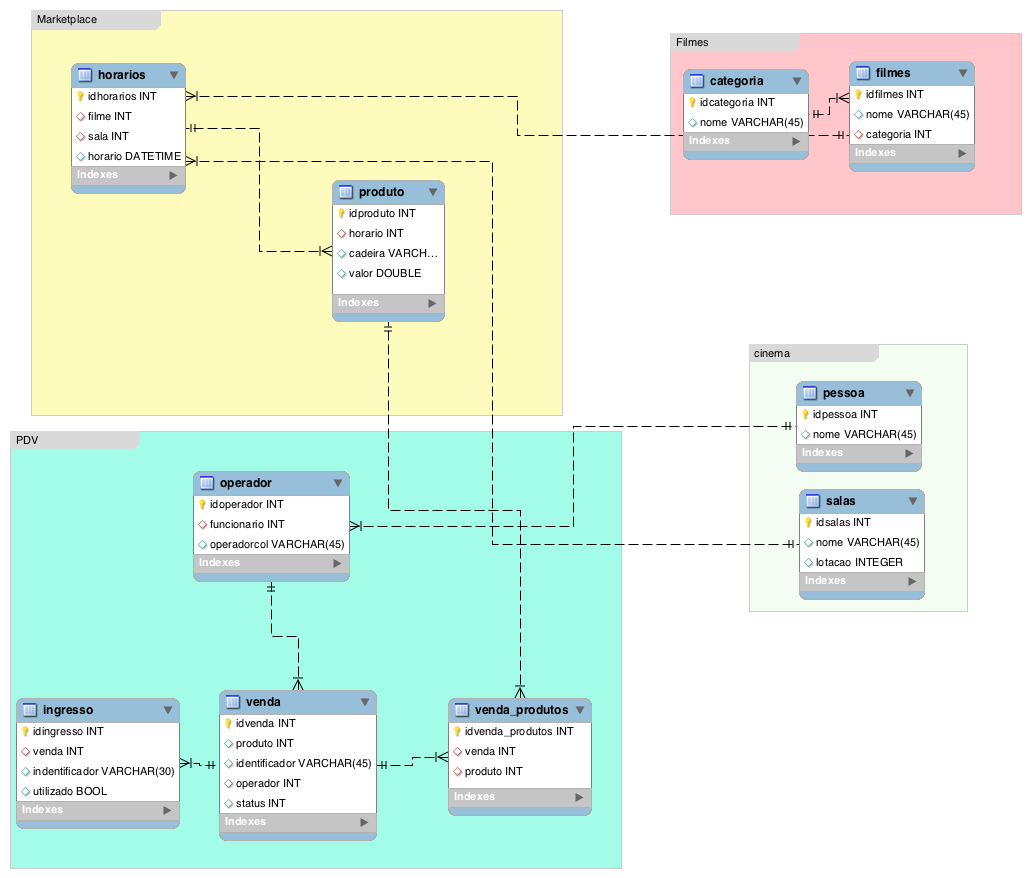
\includegraphics[width=\textwidth]{imagens/Modelo_000_Marlucio_Barbosa.png}
    \caption{Modelo Gerado pelo Participante 001}
    \label{fig:Modelo_000_Marlucio_Barbosa}
\end{figure}

\subsubsection{\hspace*{3pt} Participante 002}
\label{sec:participante_002}

O participante 002 ao ser apresentado ao contexto e a tarefa de representá-lo, pontuou algumas dúvidas acerca desta. O contexto, embora definisse o domínio, carecia de uma visão mais focada que guiasse o participante na direção de uma representação mais específica. Outra dúvida fora sobre a maneira que ele poderia representar o contexto, isto é, que ferramentas ou linguagens poderia se valer para a execução da tarefa.

Fora explicado ao participante que o mesmo deveria tomar as circunstâncias que lhe fossem mais comuns para a representação do contexto e poderia se valer de qualquer linguagem que lhe parecesse mais simples ou detivesse maior experiência de uso. Tendo esclarecido estas questões, o participante optou por utilizar a linguagem E-R, disponibilizada em uma ferramenta web para executar seu modelo.

Seguindo as orientações, o participante definiu primeiro todas as entidades que ele julgou pertinentes ao contexto na seguinte ordem: \textbf{GRUPO}, \textbf{FILIAL}, \textbf{SALA}, \textbf{LOCALIZACAO}, \textbf{SERVICO}, \textbf{FUNCIONARIO}, \textbf{FILME}, \textbf{SESSAO} e \textbf{DISTRIBUIDORA}.

Sua abordagem seguiu a visão \textit{top-down}, onde a entidade mais geral, o grupo que representa todas as salas de cinema, foi a primeira a ser definida, e cada conceito pertencente ao primeiro, fora definido um após o outro.

Após determinar todas as entidades, o participante 002 representou cada uma das relações que as entidades possuíam umas com as outras, de acordo com a sequência: \textbf{GRUPO} se relaciona com \textbf{FILIAL}, \textbf{FILIAL} com \textbf{FUNCIONARIO} e com \textbf{SALA}, \textbf{SALA} por sua vez se relaciona com \textbf{SESSAO} e \textbf{LOCALIZACAO}. Neste ponto, o participante ficou confuso quanto ao tipo de relacionamento que \textbf{SALA} manteria com \textbf{LOCALIZACAO}. Dando continuidade aos relacionamentos, o participante 002 definiu a relação entre \textbf{SESSAO} e \textbf{FILME}, \textbf{FILME} com \textbf{DISTRIBUIDORA} e \textbf{LOCALIZACAO} com \textbf{SERVICO}. 

O participante 002 precisou definir ainda as seguintes entidades \textbf{INGRESSO},  \textbf{CANAL DE VENDA} e \textbf{CONTRATO}, traçando a relação de \textbf{SESSAO} com \textbf{INGRESSO}, \textbf{INGRESSO} com \textbf{CANAL DE VENDA}, \textbf{GRUPO} com \textbf{CONTRATO}, \textbf{CONTRATO} com \textbf{DISTRIBUIDORA}.

Neste ponto, mais uma entidade precisou ser definida, \textbf{USUARIO ON LINE}, que foi relacionada com \textbf{INGRESSO}, gerando novamente dúvidas sobre o tipo de relacionamento que manteriam uma com a outra.

Como última etapa do processo de modelagem, o participante 002 definiu as características que cada entidade da seguinte maneira:

\textbf{GRUPO} (\textit{sede}, \textit{marca}, \sout{\textit{empresa}} ,\textit{cnpj}); \textbf{CONTRATO} (\textit{valor}, \textit{vigencia}, \textit{logistica}); \textbf{FILIAL} (\textit{cnpj}, \textit{responsavel}); \textbf{FUNCIONARIO} (\textit{nome}, \textit{cpf}, \textit{salario}, \textit{funcao}, \textit{cargo}); \textbf{LOCALIZACAO} ( \textit{shopping}, \textit{endereço}); \textbf{SALA} (\textit{mapa de cadeiras}, \textit{código}, \textit{3d}, \textit{imax}, \textit{conforto premium}); \textbf{DISTRIBUIDORA} (\textit{responsavel}, \textit{cnpj}, \textit{contato}); \textbf{FILME} (\textit{titulo}, \textit{classificacao}, \textit{descricao}, \textit{midia}, \textit{trailer}); \textbf{SESSAO} ( \textit{horario}, \textit{dublado/legendado}, \textit{3D}); \textbf{SERVICO} (\textit{pipoca}, \textit{promocoes}, \textit{bebida}, \textit{doces}, \textit{valor}); \textbf{INGRESSO} (\textit{beneficio meia?}, \textit{valor inteira}, \textit{data compra} \textit{forma de pagamento}*); \textbf{CANAL DE VENDA} (\textit{internet}, \textit{guiche}); \textbf{USUARIO ON LINE} (\textit{id}, \textit{nome}).

Pode se observar, porém, que na entidade \textbf{GRUPO}, o participante teve dúvidas acerca de que símbolo utilizar para representar o conceito do nome do grupo da empresa. A palavra riscada, representa o signo preterido em favor do signo escolhido, marca. A características \textit{forma de pagamento}, marcada com asterisco (*), somente foi acrescentada após as definições das características de \textbf{Canal de Vendas}, evidenciando que um conceito conectou ao outro.

A preocupação do participante 002 em demonstrar informações como distribuidora, classificação, tipo de mídia, se a cópia é dublada ou legendada, por exemplo. Pode significar uma maior experiência em relação ao contexto apresentado e sua atividade fim. Seu tempo total de execução do modelo foi de aproximadamente 20 minutos.

A Figura \ref{fig:Modelo_000_igor}, representa o modelo gerado pelo pelo participante 002 ao término da tarefa.

\begin{figure}[!ht]
    \centering
    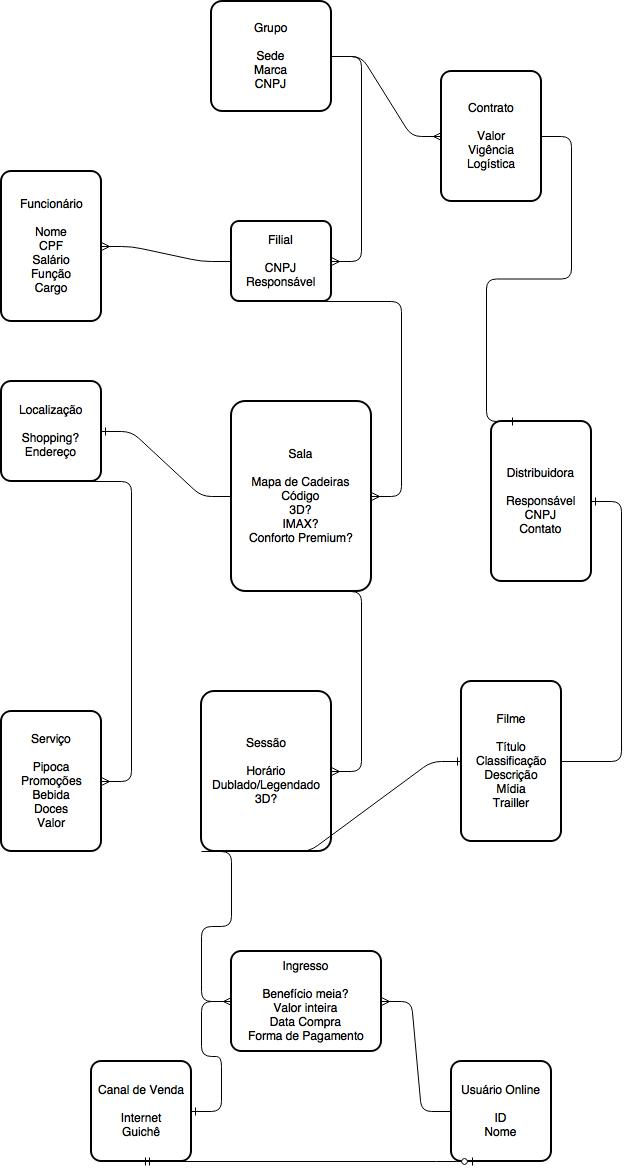
\includegraphics[width=\textwidth, height=\textwidth]{imagens/Modelo_000_Igor.jpg}
    \caption{Modelo Gerado pelo Participante 002}
    \label{fig:Modelo_000_igor}
\end{figure}

\subsubsection{\hspace*{3pt} Participante 003}
\label{sec:participante_003}

O participante 003, também ficou em dúvidas ao ser apresentado à tarefa, questionando como, exatamente, deveria efetuar o modelo. Ao qual foi esclarecido, que assim como constava nas orientações, ele deveria escolher o método para representação que se sentisse mais a vontade e que melhor demonstrasse as particularidades do contexto. Quando questionou sobre que tipo de informações deveria priorizar no modelo, lhe foi solicitado que representasse aquelas que ele julgasse necessárias para demonstrar seu conhecimento sobre a mesma, de maneira clara.

O participante 003 começou sua modelagem às 00:32, optando para executar a tarefa por uma descrição textual das entidades, relacionamentos e propriedades. A primeira entidade descrita por ele, foi \textbf{FILME}, com os atributos básicos \textit{título} e \textit{duração}. Pode-se perceber aqui a associação do conceito cinema, representando o contexto, ao conceito filme, como um conceito mais específico, conforme apresentado por \cite{dahlberg:1978.fundamentos}. A próxima entidade descrita foi \textbf{SALA}, com o atributo \textit{nome}. E depois a entidade CLIENTE, e seus atributos: \textit{nome} e \textit{endereço}, sendo essa última como uma referência para a entidade, ainda vindoura.  A próxima entidade descrita fora \textbf{FUNCIONÁRIO}, possuindo também os atributos \textit{nome} e \textit{endereço}, endereço também como referência.

A entidade \textbf{CINEMA}, foi a quarta entidade a ser descrita e continha os atributos \textit{nome}, \textit{salas} e \textit{endereço}. O símbolo escolhido para representar o conceito sala, estava na forma plural, demonstrando que o participante entende que o conceito cinema, por ser geral, pode conter mais de uma sala, mas apenas um endereço, por esse motivo a falta da forma plural deste último signo. Outro indicador de que as noções hierárquicas estão presentes na modelagem, é o fato que ambos os atributos, entraram como referencias a outras entidades.

A entidade \textbf{SESSÃO}, com os atributos \textit{horário início}, \textit{horário fim}, \textit{preço}, \textit{número total de assentos}, \textit{funcionário responsável}, como referência a entidade \textbf{FUNCIONÁRIO} foi definida. Ainda durante a definição deste conceito, o participante 003 adicionou o símbolo \textit{número}, aos símbolos \textit{total de assentos}, que representavam essa característica. 

\textbf{COMPRA}, com os atributos \textit{cliente}, \textit{sessão}, \textit{número do assento comprado} e \textit{forma de pagamento}, foram foram definidas. o atributo cliente fazendo referência para a entidade \textbf{CLIENTE} e o atributo sessão, fazendo referência para a entidade \textbf{SESSÃO}.

A entidade \textbf{AVALIAÇÃO} com os atributos \textit{compra} fazendo referência a entidade \textbf{COMPRA} e o atributo \textit{nota da avaliação}, foram descritas logo após.

O participante julgou ser preciso esclarecer a necessidade de elaboração de regras para o melhor entendimento do modelo, com por exemplo verificar a quantidade de assentos disponíveis e se um determinado filme ``caberia'' em uma sessão. 

Ao analisar os conceitos definidos, recordou-se que embora prevista, ainda não havia definido a entidade \textbf{ENDEREÇO}, que foi definida com os atributos \textit{rua}, \textit{número} e \textit{etc}. Neste momento, o participante também definiu os atributos \textit{filme} e \textit{sala}, como referências às entidades homônimas, para a entidade \textbf{SESSÃO}, por terem sido definidas em um momento posterior, assinalamos no modelo descrito com asterisco (*).

A execução da tarefa teve seu final às 00:57 e o resultado de seu modelo, por ser textual, está transcrito aqui:

\begin{quote}
FILME\\
	- Título\\
	- Duração (em minutos)\\
SALA\\
	- Nome\\
ClIENTE\\
	- Nome\\
	- Endereço (referência para entidade endereço)\\
FUNCIONÁRIO\\
	- Nome\\
	- Endereço (referência para entidade endereço)\\
CINEMA\\
	- Nome\\
    - Salas (referência para entidade salas)\\
    - endereço (referência para entidade endereço)\\
SESSAO\\
	- Horário início (data/hora)\\
    - Horário fim (data/hora)\\
    - Preço\\
    - Número de assentos disponíveis\\
    - Funcionário responsável (referência para entidade funcionário)\\
    - Filme*\\
    - Sala*\\
COMPRA\\
	- Cliente (referência para entidade cliente)\\
    - Sessão (referência para entidade sessão)\\
    - Número do assento comprado\\
    - Forma de pagamento\\
AVALIAÇÃO \\
	- Compra (referência para entidade compra)\\
	- Nota da avaliação\\
ENDEREÇO \\
	- Rua \\
    - Número \\
    - Etc \\
\end{quote}

\subsubsection{\hspace*{3pt} Participante 004}
\label{sec:participante_004}

Após a explicação da tarefa, o participante em dúvida, questionou acerca da abordagem que deveria seguir para representar o contexto, ao qual foi respondido que deveria seguir aquela que ele julgasse mais adequada para representar o contexto, seguindo sua experiência e interação com o mesmo. 

O participante 004 iniciou sua modelagem às 18:24 e escolheu como ferramenta para auxiliá-lo o programa Astah, no qual optou por fazer um modelo de diagrama de classes. Sua abordagem de modelagem, seguiu a abordagem \textit{top-down} cuja entidade inicial do modelo recebeu o nome do contexto ao qual ele procurava representar, isto é, \textbf{CINEMA}. Na sequência, as entidades \textbf{UNIDADE}, \textbf{ENDERECO} e \textbf{SALA}, e suas relações foram definidas, antes que o participante seguisse na busca de outras entidades.

As entidades definidas na sequência foram: \textbf{ASSENTO}, \textbf{SESSAO} e \textbf{FUNCIONARIO}, assim como suas relações com as entidades já definidas. Nesta avaliação, foi possível notar a influência que a entidade \textbf{SALA}, exerceu na definição das entidades seguintes, assim como nas relações que as novas entidades mantinham com entidade \textbf{SALA}. Percebeu-se que, após a definição da entidade \textbf{FUNCIONARIO}, o participante precisou rememorar suas experiências e comparar com o que estava representando, pois o mesmo não adicionou nenhuma alteração ao modelo por um período longo de tempo, se comparado à performance que estava desenvolvendo até então. Após o período de rememoração, o participante definiu a entidade \textbf{FILME} e a relacionou com a entidade \textbf{SESSAO}, entrando novamente em estado de rememoração.

O próximo passo do participante foi definir os atributos das entidades definidas. Ficou evidente que as características definidas foram àquelas que o participante tinha conhecimento e julgou necessário de acordo com o contexto abordado, por exemplo os atributos \textit{horaInicial} e \textit{horaFinal} para a entidade \textbf{SESSAO}. Durante a definição dos atributos, o participante percebeu a necessidade de uma nova entidade, a qual ele nomeou \textbf{FUNCAO} e a associou as entidades \textbf{UNIDADE} e \textbf{FUNCIONARIO}. 

Duas outras entidades foram definidas em seguida: \textbf{ESTOQUE} e \textbf{PRODUTO}, assim como suas relações. A ordem da definição das entidades, seguindo as experiências demonstradas por \citeonline{rosch:1975.family}, apontam para a possível ordem que o participante habitualmente interage com o contexto, no qual a \textit{bomboniere} é o ultimo local visitando, antes de entrar na sala para uma sessão de cinema.

O processo de modelagem do participante 004 terminou às 19h, a Figura \ref{fig:Modelo_000_wagner} representa o modelo gerado pela atividade.

\begin{figure}[!ht]
    \centering
    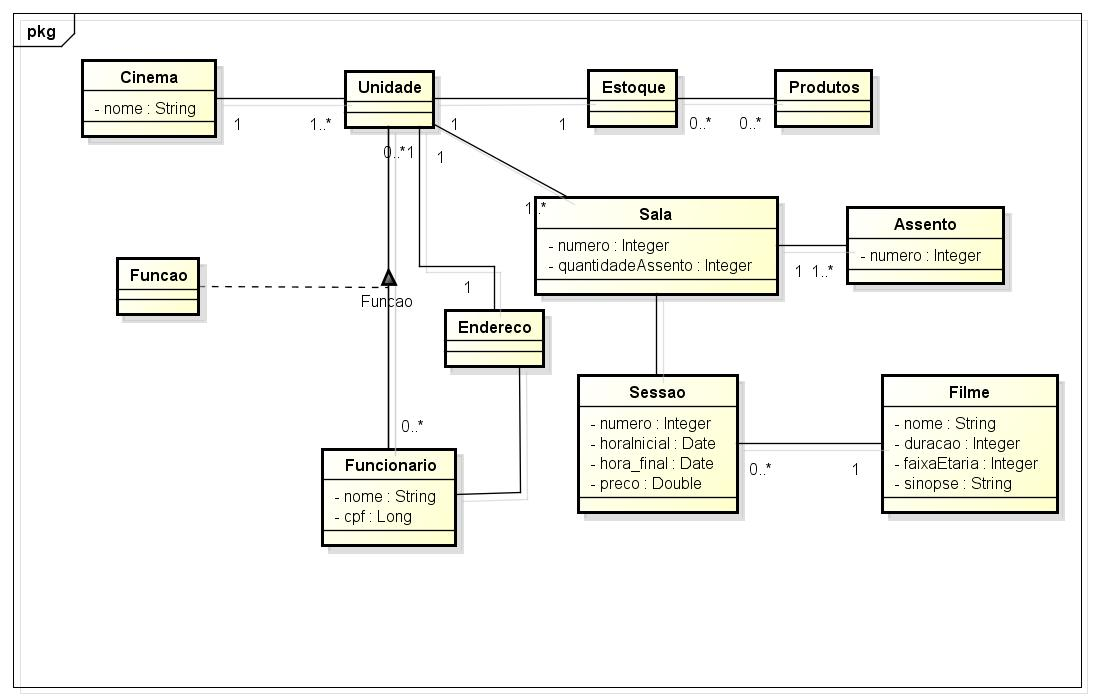
\includegraphics[width=\textwidth, height=\textwidth]{imagens/Modelo_000_Wagner.jpg}
    \caption{Modelo Gerado pelo Participante 004}
    \label{fig:Modelo_000_wagner}
\end{figure}

\subsubsection{\hspace*{3pt} Participante 005}
\label{sec:participante_005}

Ao ser apresentado à tarefa, o participante 005 questionou sobre o tipo de abordagem que deveria seguir. Ao ser indagado sobre a natureza de sua dúvida, o mesmo respondeu que necessitava saber mais sobre o contexto para poder modelá-lo. Ao participante, fora explicado que fazia parte do da pesquisa aferir que abordagem ele escolheria, assim como a maneira que iria implementá-la. Para tal, ele deveria seguir a abordagem que lhe parecesse mais adequada para representar seus conhecimentos sobre o contexto. 

Depois de optar pela linguagem UML e seu diagrama de classes, utilizando papel e lápis, começou a definir as entidades que, segundo ele, representavam sua visão sobre o contexto.

A primeira entidade definida pelo participante fora \textbf{FILME} com os atributos \textit{nome}, \textit{duracao}, \textit{genero}, \textit{produtora} e \textit{atores}. Seguida da entidade \textbf{CINEMA}, possuidora dos atributos \textit{endereco}, \textit{cnpj}, \textit{nome-social} e \textit{telefone}. Percebe-se pelos atributos definidos para a entidade filme, que o participante possui uma afinidade maior com a atividade fim do contexto, se comparado ao demais participantes desta fase, dado o grau de detalhamento que o mesmo dedicou a entidade, e possivelmente a mais importe, pois as demais entidades surgiram em natural associação com as primeiras, por exemplo a entidade \textbf{SESSAO} e seus atributos \textit{data}, \textit{hora} e \textit{numero de identificacao}. 

A entidade \textbf{EMPREGADOS} foi definida em seguida, mantendo ligação com a entidade \textbf{CINEMA}, e para esta entidade o participante definiu os atributos \textit{nome}, \textit{cpf} e \textit{telefone}, determinando a partir desta relação a entidade \textbf{INSCRICAO} com os atributos \textit{numero de identificação} e \textit{sede}.

O processo de modelagem do participante, demorou 4 minutos no total, e a Figura \ref{fig:Modelo_000_modesto} representa o modelo criado.

\begin{figure}[!ht]
    \centering
    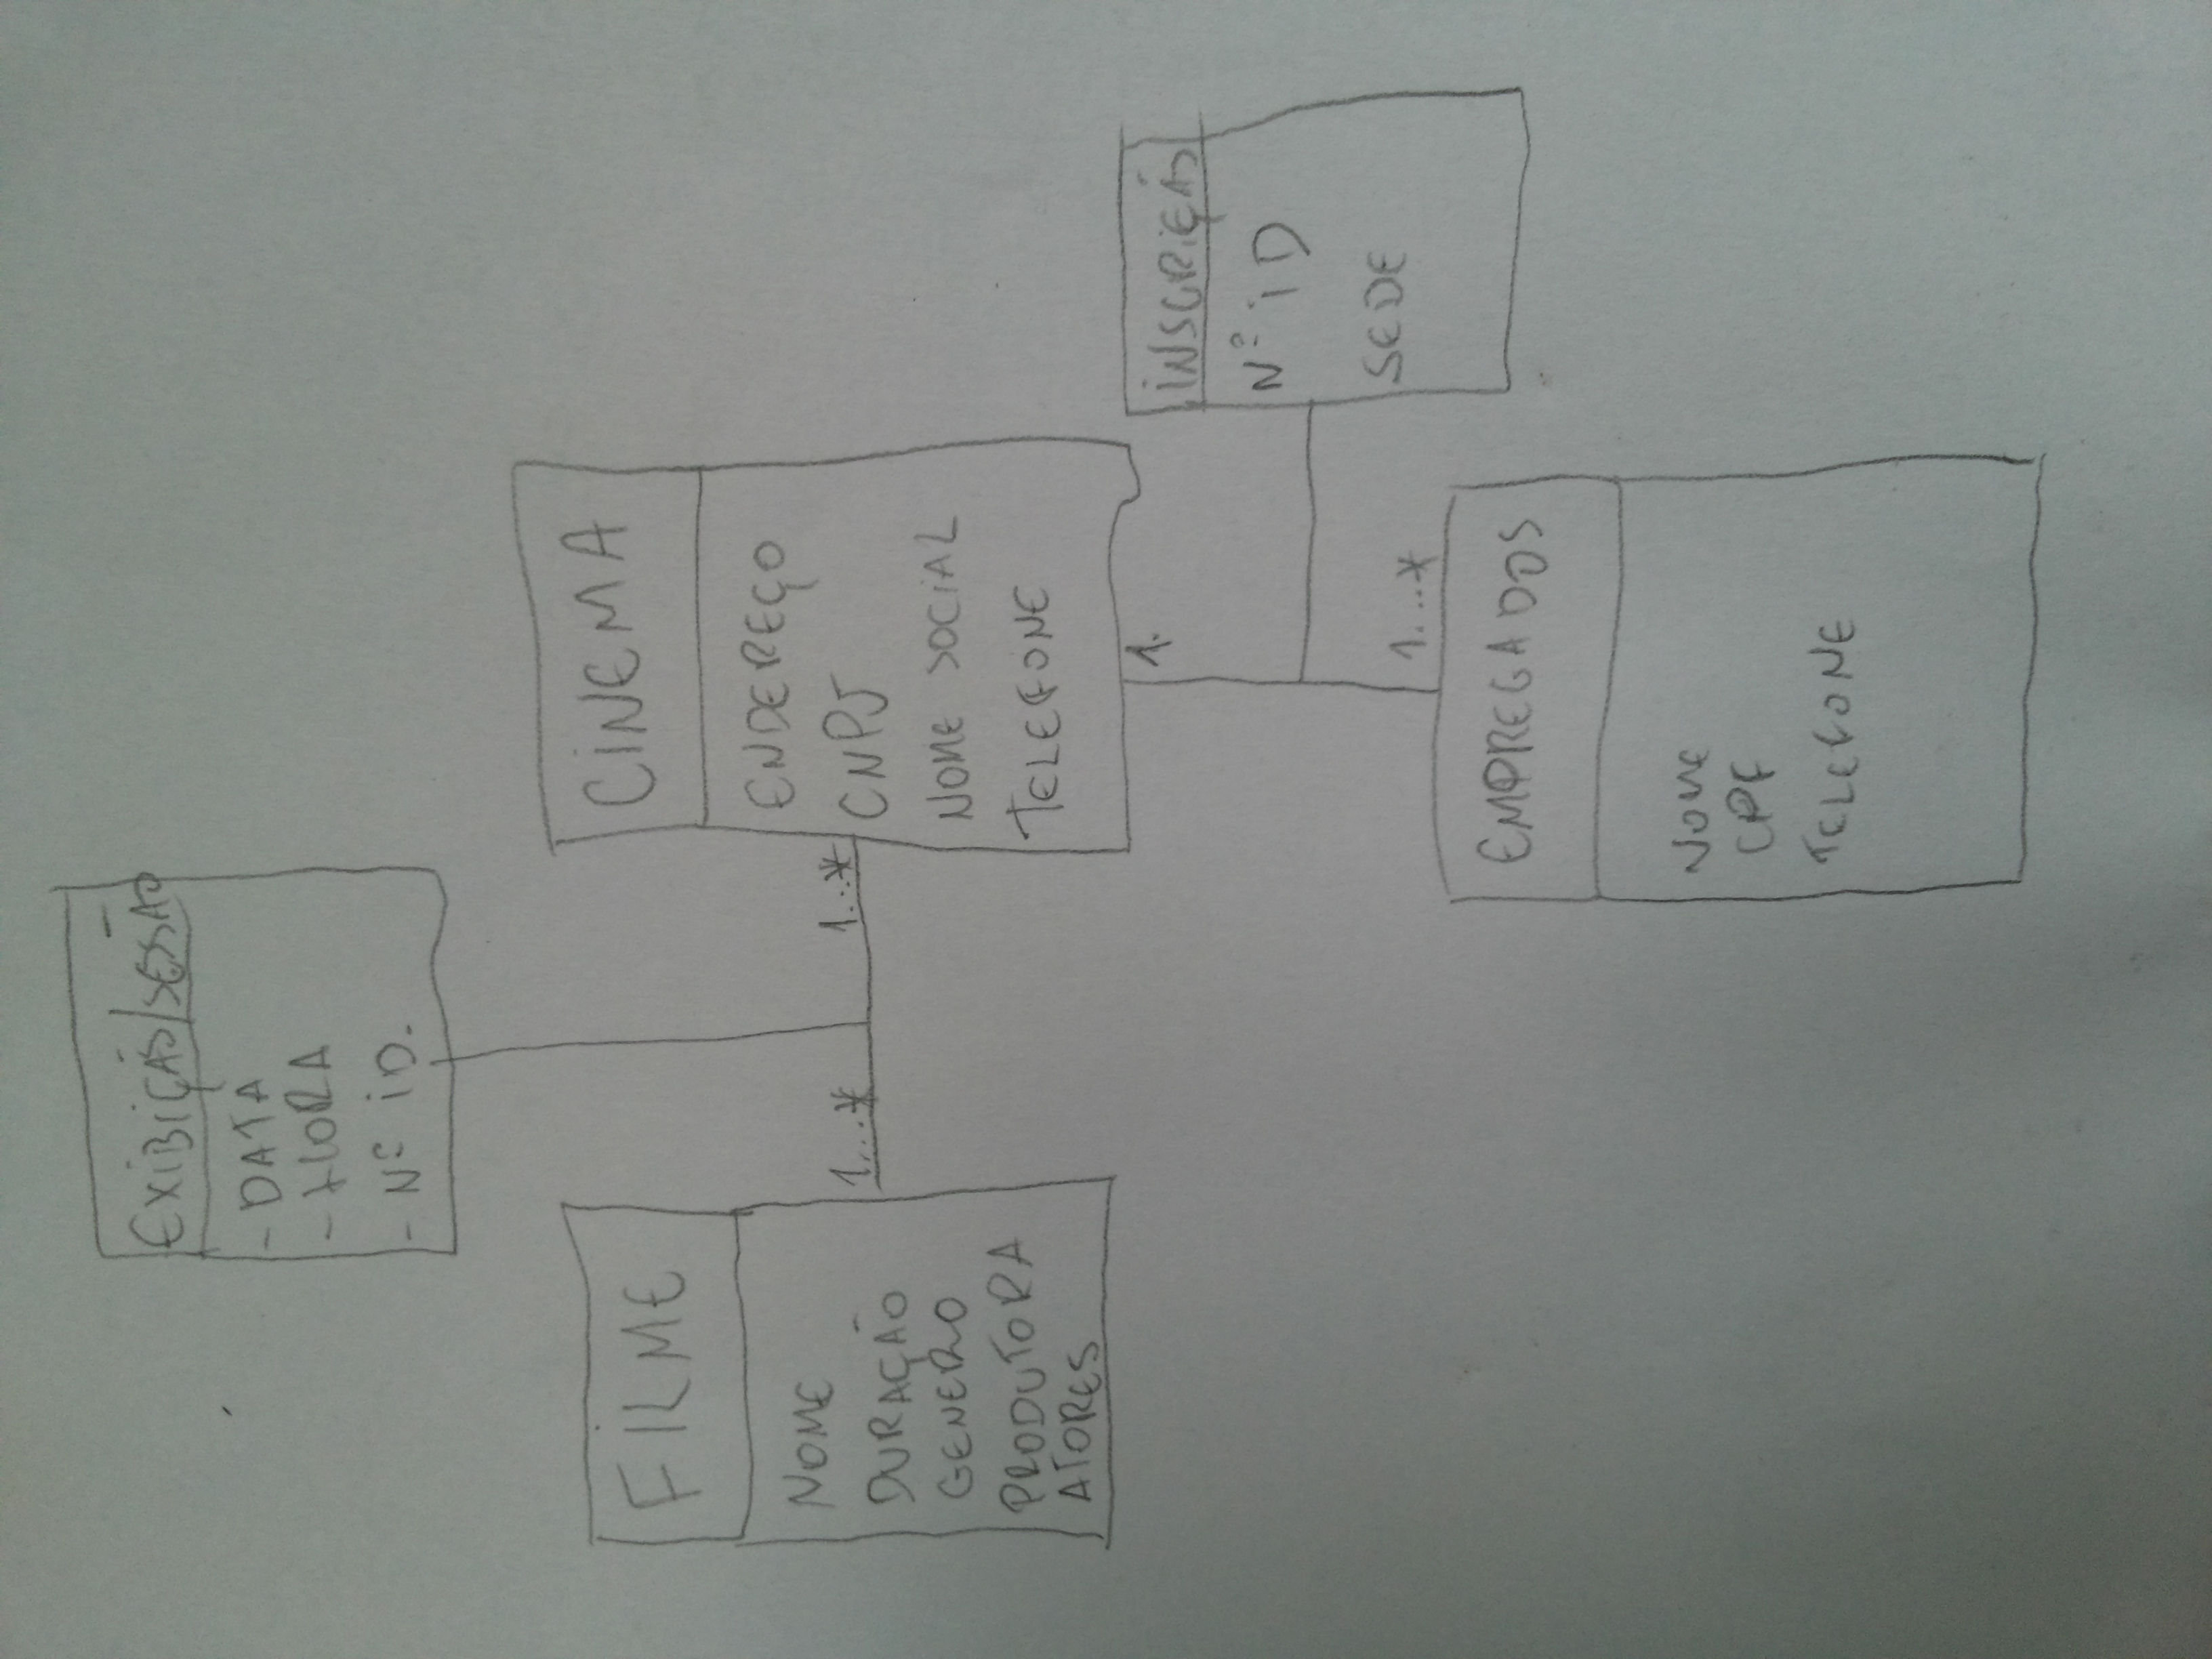
\includegraphics[width=\textwidth, height=\textwidth,angle=270]{imagens/Modelo_000_Modesto.jpg}
    \caption{Modelo Gerado pelo Participante 005}
    \label{fig:Modelo_000_modesto}
\end{figure}

\section{\hspace*{3pt} Conclusão}
\label{sec:conclusaoModeloConceitual}

Durante os processos de modelagem, a abordagem \textit{top-down}, prevaleceu em todos os casos, o que pode ser um reflexo da categorização automática. 

Se pôde observar que conceitos que são mais comuns no contexto de um cinema (filme, ingresso, horário e sala) foram identificados de maneira mais rápida e direta. Algumas características como diretor, ator, gênero, classificação etária, por exemplo, não foram abordadas por todos participante, o que pode significar que nem todos usuários observam estas características quando se utilizam dos serviços oferecidos pelo domínio.

No entanto, são conceitos que poderiam ser facilmente associados aos modelos elaborados se, como sugere \citeonline{dahlberg:1978.fundamentos}, o conceito filme fosse definido buscando-se as características que o definem e compõe. É fácil observar que, mesmo em um contexto onde o cinema é visto como um lazer despretensioso, atores e diretores figuram como características importantes, sendo estampados em cartazes afim de atrair público, por exemplo. 

Não seria forçoso assumir que para frequentadores de cinema, ao menos em algum momento, um filme fora escolhido por ter um determinado ator ou atriz como protagonista. Neste quesito, não podemos ignorar o papel que conceitualizações prévias acerca deste ou aquele ator, teriam ao se formar esse conceito, pois como definido por \citeonline{kant:1983.critica}, a faculdade de juízo carece de uma recionalização baseada em categorias já conhecidas, neste caso, as qualitativas - ser bom ator, por exemplo. 

Processos mais operacionais do ponto de vista negocial, tais como vendas dos produtos e dos próprios ingressos, embora tenham sido alcançados, demonstraram uma maior dificuldade para serem representados, reflexo da baixa interação dos participantes com os processos internos do negócio. 

No entanto, novamente argumentamos que estes mesmos processos são, na verdade, conhecidos pelos participantes, pois todos que já interagiram com a atividade de compra, mesmo como consumidor, conhece suas etapas. Um paralelo entre as características já dominadas em outras atividades de compras, com os processos de aquisição de ingresso e produtos, poderia ser estabelecido afim de que a representação desses processos pudesse ser representado. 

Um processo que levasse o modelador a refletir sobre os conceitos que já domina e quais as características que lhe dão a certeza desta convicção, isto é, quais as características que definem o conceito , poderia facilitar o entendimento de diferentes contexto que compartilhassem conceitos semelhantes.          
        %A literatura demonstraque a racionalização do conhecimento é uma área fértil para perspectivas e abordagens distintas. No entanto acreditamos que, no âmbito da elaboração de modelos conceituais, uma maneira de representar o conhecimento, e perceber os pontos de convergência entre essas teorias pode fornecer um ponto de apoio no processo de representação conceitual acerca de um determinado domínio.

Neste propósito, defendemos que é preciso um processo que seja capaz de guiar os modeladores através dos pontos de convergência de maior destaque. Evidenciar a discussão inerente ao processo de construção de modelos conceituais, passando de maneira ativa por cada uma das etapas identificadas e discutidas nas abordagens que servem de fundamentação para este trabalho.

Com base nas teorias apresentadas neste trabalho, elaboramos um fluxo que visa auxiliar a elaboração de modelos conceituais. O processo proposto contempla fases que possuem como propósito guiar o modelador na busca acerca do seus conhecimentos sobre o contexto e como sucedeu sua aquisição. Tal busca, intenciona refletir na sua representação mais expressiva e completa.

Este processo, embora esteja dividido em três fases (Percepção, Racionalização e Representação), apresenta sua discussão centrada na fase 2, a racionalização, pois entendemos que esta fase contém o ponto crítico do processo de raciocínio e representação do conhecimento. Em cada fase, identificamos uma ou mais etapas que irão compor o fluxo, que serão apresentadas nas seções seguintes.

A figura 9 representa essas etapas resumidamente.


Fases do Processo Objeto-Representação



4.1. Fase 01: Percepção

A fase 01 foi definida como a Percepção, cuja função é fornececer os objetos que serão racionalizados.

Objeto é tudo aquilo que nos circunda ou é designado pelo homem; são as ``coisas" do mundo. Nesta dissertação, o termo "objeto" é empregado de maneira ampla e pode representar tanto objetos concretos (ex.: um animal ou um veículo), quanto objetos abstratos (ex.: um departamento ou um dragão)(Dahlberg, Ingetraut, 1978; Machado, Felipe Nery Rodrigues; Abreu, Maurício Pereira de, 2009).

Podemos, ainda, categorizá-los em objetos sensíveis, isto é, aqueles objetos que são evidenciados para nós através de um, ou mais, sentidos e objetos inteligíveis, cuja sensação é fruto de um processo mental, como por exemplo a junção de ideias de mulher e peixe, para formar uma sereia ou conceitos que não existem de maneira física, como sentimentos.

Ao categorizar os objetos em sensíveis e inteligíveis, apesar de reconhecer toda a batalha filosófica travada ao longo dos séculos entre as correntes denominadas Empirismo, Racionalismo e Criticismo, não estamos assumindo uma postura Empirista, mas queremos apenas evidenciar os objetos abstratos, como frutos de um processo racional e reflexivo, a despeito de quaisquer discussões filosóficas subjacentes.

A base da percepção humana são os sentidos, sendo estes estimulados de maneira contínua por um fluxo de acontecimentos. Disto resulta uma excitação neural chamada de sensação(Alexandre, Dulclerci Sternadt; Tavares, João Manuel R. S., 2007).

Sensação, segundo o dicionário onlinePriberam, (2015), é "a impressão produzida pelos objetos exteriores num órgão dos sentidos, transmitida ao cérebro pelos nervos, onde se converte em ideia, julgamento ou percepção".

Na introdução da Crítica da Razão Pura,Kant, Imanuel, (1983) afirma que:

"Não há dúvida de que todo o nosso conhecimento começa com a experiência; do contrário, por meio do que a faculdade de conhecimento deveria ser despertada para o exercício senão através de objetos que toquem nossos sentidos e em parte produzem por si próprios representações, em parte põem em movimento a atividade do nosso entendimento para compará-las, conectá-las ou separá-las e, desse modo, assimilar a matéria bruta das impressões sensíveis a um conhecimento dos objetos que se chama experiência? […]"(Kant, Imanuel, 1983).
Estas impressões, no entanto, são percepcionadas no espaço e no tempo, uma vez que formas puras (vazias) fazem parte das estruturas cognitivas inatas do sujeito. Elas são a condição indispensável para que possamos ter acesso ao conhecimento, isto é, a sensibilidade expressa-se em duas formas: espaço e tempo, os quais, nas palavras de Kant, Imanuel, (1983), são definidos, respectivamente, como:

"O espaço não é um conceito empírico abstraído de experiências externas. Pois a representação de espaço já tem que estar subjacente para certas sensações se referirem a algo fora de mim […] O espaço é uma representação a priori necessária que subjaz a todas as intuições externas. […] O espaço não é um conceito discursivo ou, como se diz, um conceito universal de relações das coisas em geral, mas sim uma intuição pura. […] O espaço é representado como uma magnitude infinita dada. […] A representação originária do espaço é, portanto, intuição a priori e não conceito" (Kant, Imanuel, 1983)
"O tempo não é um conceito empírico abstraído de qualquer experiência. […] O tempo é uma representação necessária subjacente a todas intuições. […] Sobre essa necessidade a priori também se funda a possibilidade de princípios apodíticos das relações do tempo, ou de axiomas do tempo em geral. […] O tempo não é um conceito discursivo ou, como se diz, um conceito universal, mas uma forma pura da intuição sensível. […] A infinitude do tempo nada mais significa que toda magnitude determinada do tempo só é possível mediante limitações de um tempo uno subjacente" (Kant, Imanuel, 1983)
O espaço e o tempo não são conceitos, visto que não são elaborados pelo sujeito tendo como ponto de partida suas experiências; eles simplesmente existem no sujeito cognoscente, que ao conhecer os objetos do mundo, o fazem de um modo dimensionado e associado à ideia de movimento, de mudança, de evolução, ou mesmo em estágios ou locais diferentes. Por isso as noções de espaço e de tempo são condições necessárias para o conhecimento dos objetos do mundo.

É através de sua percepção que um indivíduo organiza e interpreta suas impressões sensoriais para atribuir significado ao seu meio. Do ponto de vista cognitivo, a percepção envolve processos mentais que interpretam os dados oriundos dos sentidos e os associam aos conceitos.

4.2. Fase 02: Racionalização

A racionalização permite-nos dar significados aos estímulos que recebemos, transformando os dados oriundos das percepções em ideias ou conceitos.

Esta fase compartilha a visão atomística, que defende que a compreensão de um objeto implica o reconhecimento das partes para ter o entendimento do todo. Embora a visão holística - aquela que defende que a interpretação de um objeto se dá pelo todo - seja reconhecida, o todo quando inserido em um contexto, pode apresentar características que não sejam relevantes para a conceitualização do objeto.

Os experimentos propostos porRosch, Eleanor, (1999), para encontrar o nível médio de abstração: atributos comuns, movimentos motores, forma objetiva e semelhança da forma, ou as forma de conhecer o mundo, quando dentro do contexto, permitem que identifiquemos quais características são importantes para definição do objeto.

O contexto delimita, no universo do nosso discurso, quais as características dos objetos que percebemos fazem sentidos, e precisam ser compartilhadas para que nossas representações tenham sentidopara nossos interlocutores. 

A categorização reflete a nossa capacidade para agrupar entidades únicas em conjuntos, usando como regras de agrupamento as características que compartilham entre si.

4.2.1. Formas de Conhecer o Mundo

Atributos comuns são as características que dois ou mais objetos de uma mesma categoria compartilham. Ex.: ter bicos, ter penas, por ovos.

Movimentos motores representam a maneira como interagimos com determinados objetos, os movimentos musculares associados à utilização do objeto. Ex.: o ato de sentar em uma cadeira ou de cortar com um serrote.

Formas Objetivas e Similares dizem respeito à forma como o objeto se apresenta, isto é, a forma que ele possui. Ex.: cadeira de jantar, cadeira de praia, poltrona.

Nossa experiência associa características novas àquelas percebidas previamente, que sejam semelhantes. Refletir acerca da maneira como as características nos chegam nos ajudam a entender como estamos categorizando um determinado grupo de características.

4.2.2. Contexto

É o contexto que define o universo do discurso, influencia os conceitos que serão utilizados para expressarem um grupo de objetos ou relações. Segundo Olson, Hope A., (2012), a relevância do contexto para a nossa capacidade de interpretar o que percebemos não é uma fantasia filosófica acadêmica esotérica; É o que fazemos todos os dias. Ex.: Podemos falar de cinema, enquanto empresas de exibição de filmes de cinema; ou de cinema do ponto de vista da indústria que produz imagens com impressão de movimento, contendo narrativa.

Podemos afirmar então, que o ato de categorizar passa a ser encarado como um processo interacional, construído de maneira discursiva e dependente de um contexto(Carvalho, Maria de Lourdes Guimarães de; Souza, Mariléia de, 2013).

Vickery, Brian Campbell, (1980), citado por Silva, Alessandra Rodrigues da; Lima, Gercina Ângela Borém, (2011), reforçando essa ideia diz:

"A aquisição do conhecimento é um processo ativo. É uma interação concreta entre o organismo humano e seu ambiente, no curso do qual o ambiente é física e objetivamente mudado, e o organismo é também mudado, mas mental e subjetivamente. Estudando o desenvolvimento das categorias conceituais, não são apenas as atividades mentais como ‘a distinção’ que devem ser levadas em consideração. A atividade total, mental e física é envolvida (Vickery, Brian Campbell, 1980).
Medrado, Betânia Passos, (2008), afirma que o contexto traz além dos aspectos linguísticos, elementos corporais, gestuais, identidades institucionais e papéis sociais, ou seja, elementos socioculturais, produzindo uma relação dinâmica entre linguagem, cognição e interação(Carvalho, Maria de Lourdes Guimarães de; Souza, Mariléia de, 2013).

4.2.3. Categorização

Uma das formas que a categorização pode se dar, segundoRichardson, Roberto Jarry; Peres, José Augusto, (1985), é como o resultado da classificação progressiva dos elementos. A maior parte deste processo de categorização ocorre automática e inconscientemente, este processo só se torna perceptível a nós quando ocorrem casos dúbios. Oferecemos uma maneira de pensar sobre os conceitos e construir gradualmente o sistema de categorias que irão comportar os conceitos, conscientemente.

O significado linguístico está estreitamente relacionado com os processos de categorização, ``os conceitos, os significados não são, pois, rótulos das coisas nem objetos mentais aprioristicamente dados, mas categorias e, como tal, criações da cognição humana que servem para dar sentido ao mundo”(da Silva, Augusto Soares, 2006).

Categorizar é agrupar entidades (objetos, ideias, ações, etc) por semelhança(Lima, Gercina Ângela Borém, 2007). Este é um processo mental habitual ao homem, pois vivemos automaticamente classificando ideias e coisas a fim de compreender e conhecer a realidade(Piedade, Maria Antonieta Requião, 1983).

A Figura 10 desdobra a fase de Categorização/Conceitualização.


Fases do Processo Objeto-Representação (Estendido)
4.2.3.1. Características

Dahlberg, Ingetraut, (1978) define característica como uma unidade de conhecimento. Cada conceito é então entendido como um conjunto de características necessárias para a sua definição, e cada característica pode ser definida como um enunciado verdadeiro acerca do objeto(Dahlberg, Ingetraut, 1978).

Enunciado é qualquer frase ou oração, que exprima um pensamento de sentido completo, isto é, aquele pensamento que admite apenas um dos valores verdadeiro (V) ou falso (F). Mas para nossos propósitos, consideraremos apenas as frases declarativas cujo valor de verdade possa ser asseguradamente o verdadeiro (V).

Pelo fato de os enunciados sobre um objeto serem tão vastos, quanto nossos conhecimentos permitam, podemos tomar como exemplo a tabela categorial de Aristóteles, a fim de permitir a identificação do maior número de características possíveis.

As categorias Aristotélicas, apresentadas na Tabela 1, foram escolhidas como base neste trabalho, primeiro por entender a importância de sua classificação categórica para as teorias subjacentes e segundo por seguir a proposta deDahlberg, Ingetraut, (1978).

Categorias de Aristóteles
Categoria	Descrição	Exemplo
Matéria	É o que existe em si mesmo, o próprio objeto e seu material de origem	de pedra, de madeira, de vidro, etc.
Qualidade	É a determinação da matéria da substância, atribuindo-lhe partes distintas de outras partes.	possuir determinada estrutura, determinada forma, ser redondo, denso, colorido etc.
Quantidade (Extensão)	É a determinação da natureza ou da forma da substância.	possuir comprimento, largura, peso etc.
Relação	É a referência que um objeto ou uma característica possui com uma outra.	ser o dobro, ser mais largo, ser causa de, ser condição de, etc.
Processo (atividade, ação)	É o exercício das faculdades ou de poder sobre o objeto, de modo a produzir um efeito em alguma outra coisa ou nele mesmo.	começar, continuar, terminar, realizar algo etc.
Modo de ser	É posição relativa que as partes de um conceito têm quanto às outras.	estar em pé, sentado, voando, etc.
Passividade (paixão)	É a recepção sofrida, por um conceito, de um efeito produzido por algum agente.	ser cortado, pressionado, etc.
Posse (hábito)	Consiste em roupas, ornamentos ou outras posses.	usa sapatos, está armado, etc.
Localização (lugar, espaço)	É posição em relação aos corpos que circundam uma substância, que mede e determina o seu lugar.	estar em Brasília, no Rio de Janeiro, etc.
Tempo	É posição em relação ao curso de eventos extrínsecos, e que mede a duração de uma substância.	em fevereiro de 1978, etc.
A emissão de enunciados utilizando a tabela das categorias objetiva clarificar características que de outra maneira poderiam passar desapercebidas e evidencia, com maior facilidade, características simples. Sua utilização, no entanto, não tem a intenção de ser um fator limitante ou definitivo para a enunciação das características.

As formas de conhecer, propostas emRosch, Eleanor, (1999), justificam a apreensão do conhecimento para cada um dos enunciados acerca das categorias, de maneira que é possível relacionar cada categoria a pelo menos uma forma de conhecer, conforme Tabela 2.

Modos de Percepção do mundo x Categorias Aristotélicas

Atributos Comuns	Movimentos Motores	Formas Similares
Qualidade	X	X	X
Quantidade	X	X	X
Relação	

X
Processo	
X	
Modo de Ser	
X	
Passividade	
X	
Posse	
X	X
Localização	X	X	X
Tempo	X	X	X
Os enunciados podem conter características essenciais ou acidentais. Dahlberg, Ingetraut, (1978) define as características essenciais, como aquelas que definem o próprio conceito, por isso necessárias, e acidentais aquelas cuja a remoção não afetariam a categorização do objeto, por isso contingente.

Neste sentido, o contexto tem um papel importante, delimitando quais enunciados são essenciais para um determinado conceito. Embora a importância das características acidentais não sejam ignoradas, assim comoMedrado, Betânia Passos, (2008), consideraremos que apenas os enunciados necessários serão listados, quando o objeto está inserido no contexto.

Para evidenciar esse ponto, consideremos um carro (o objeto) que necessita de reparos elétricos (o contexto). Para este contexto, é irrelevante saber o tipo de combustível que o carro utiliza ou quantos quilômetros este mesmo carro é capaz de rodar com um litro de gasolina.

As características podem ainda ser simples ou complexas. Características simples dizem respeito a um único atributo. Ex.: azul, quadrado. Enquanto as complexas, usualmente, apresentam duas propriedades, ou mais, com alguma relação entre si. Ex.: pintado com tinta azul, moldado na forma quadrada. Em ambos os casos uma relação de processo(Dahlberg, Ingetraut, 1978).

4.2.3.2. Relações

Campos, Maria Luiza de Almeida, (2004) ressalta a importância das relações entre os objetos em um dado contexto, alegando que estas relações formam as estruturas conceituais deste contexto e que as mesmas possuem natureza diversa. Seguindo a definição deDahlberg, Ingetraut, (1978), para definição de conceitos, temos também a possibilidade de verificar as relações existentes entre as características de um conceito. Com esse propósito, ela define:

"Devemos estabelecer, desde logo, distinção entre as relações formais e as relações materiais, sendo que as primeiras se baseiam na comparação das características, tornando-se particularmente importantes quando se trata da compatibilidade dos conceitos e dos respectivos sistemas. As segundas têm por base o conteúdo das mesmas características. (Em síntese, deve ficar claro que as características são também conceitos, mas apenas em relação aos conceitos de que se tornaram elementos é que assumem o papel de características de conceitos)" (Dahlberg, Ingetraut, 1978).
Machado, Felipe Nery Rodrigues; Abreu, Maurício Pereira de, (2009) definem relacionamento como o fato, o acontecimento que une dois, ou mais, objetos do mundo real. As características atribuídas a diferentes conceitos nos guiará a uma análise acerca das relações entre estes conceitos.

A tabela 3, apresentada emDahlberg, Ingetraut, (1978), mostra os tipos de relacionamentos lógicos, através dos quais podemos definir as relações entre as características comuns. E através dos quais é possível estabelecer comparações entre os conceitos de modo a organizá-los.

Relacionamentos Lógicos
Relacionamento	Exemplo	Descrição
Identidade	A (x,x,x) e B (x,x,x)	As características são as mesmas;
Implicação	A (x,x) e B (x,x,x)	O conceito A está contido no conceito B;
Interseção	A (x,x,o) e B (x,o,o)	Os dois conceitos coincidem algum elemento;
Disjunção	A (x,x,x) e B (o,o,o)	Os conceitos se excluem mutuamente. Nenhuma característica em comum;
Negação	A (x,x,o) e B (o,x,o)	
O conceito A inclui uma característica cuja negação se encontra em B;

As relações lógicas desempenham um papel importante à medida que auxiliam a estabelecer comparações entre os conceitos, de modo a organizá-los nos seguintes relacionamentos semânticos: Relação de Hierarquia, Relação Partitiva, Relação de Oposição e Relação Funcional.

Relação Hierárquica (implicação) objetos que possuem características idênticas, porém um permite a ideia de um conceito mais geral que outro, então entre eles se estabelece a relação hierárquica ou relação de gênero e espécie. Pode-se então falar de conceitos mais amplos ou mais restritos. Pode-se também falar de conceito superior e inferior. O conceito superior é o mais genérico e o inferior é o mais específico(Dahlberg, Ingetraut, 1978).
Ex.: Mamífero → Cão → Pastor-Alemão

Relações hierárquicas, podem ser estabelecidas entre conceitos específicos do mesmo gênero, e recebem o nome de relações coordenadas, ou relações horizontais.
Ex.: Cão → Cão de Pequeno Porte → Pinscher, Chihuahua, Basset
.....Cão → Cão de Grande Porte → Fila, Labrador, Dálmata

Relação Partitiva existe entre dois ou mais conceitos, sendo um deles constituído por um outro. A observação de como um objeto se constitui, isto é, quais são suas partes (Campos, Maria Luiza de Almeida, 2001).
Ex.: árvore→ raízes, tronco, galhos, folhas, flores, frutos.

Relação de Oposição (negação) pode ser das seguintes espécies:
Contradição. Ex.: numérico - não numérico, presente - ausente
Contrariedade. Ex.: branco - preto

Relação Funcional (intersecção) estas relações aparecem quase exclusivamente na dependência do conceito de processo, ou seja, quando do conceito de processo deriva uma função a ele inerente. Ex.: Pintura (tem como consequência a existência de) quadros (que, por sua vez, supõe um) pintor (assim como de) críticos de arte (ou mesmo de) compradores de quadros, etc.

Será fácil verificar que as relações hierárquicas e as relações partitivas se aplicam principalmente a conceitos que expressam objetos. As relações de oposição se aplicam principalmente a conceitos que expressam características. Já as relações funcionais se aplicam sobretudo a conceitos que expressam processos(Dahlberg, Ingetraut, 1978).

4.2.3.3. Conceito

Antes mesmo da nossa capacidade da fala e da linguagem, já possuíamos a capacidade de atribuir significado às coisas. O conceito, desta forma, antecede a representação(Edelman, Gerald M, 1995) apud(Lacerda, Naziozenio Antonio, 2012). REVER

A formação do conceito dar-se-á em dois níveis, no nível individual onde as características são analisadas para que se defina os tipo de relações que mantêm entre si, e no nível contextual, onde um conceito é comparado com outro, então partindo de suas relações, sua correta intensão ou extensão seja definida, evidenciando o conceito mais adequado para representar.

Tomemos como exemplo um carro. Possivelmente a palavra escolhida para representar o conceito, por si só trouxe uma significância relevante. Porém listar as características deste único carro poderia ser uma tarefa extenuante e improfícua. Extenuante pois o número de enunciados que poderia proferir são inúmeros, e improfícuo porque sem determinar o contexto, esses enunciados podem não ter relevância. Desta forma, definiremos o contexto como sendo o de uma locadora de veículos.

Dentro deste contexto, considerando a atividade circunstancial de locar um carro, nosso escopo de características fica mais acessível. Onde podemos enunciar: seu modelo, cor, tipo de câmbio, quantidade de passageiros, tipo de combustível, tamanho da mala, quilometragem por litro, valor, se é aluguel por quilômetro rodado ou por dia, valor do seguro, etc. Apenas para citar algumas características.

A comparação do conceito carro com outros conceitos, talvez demonstre que na verdade seja melhor representar um veículo, ou ainda que esse conceito se relacionará com o funcionário e com o locatário, e que o funcionário talvez seja alguém mais específico.

4.3. Fase 03: Representação

A última etapa, a representação é a forma como escolhemos exteriorizar o conceito racionalizado. Usualmente essa forma de expressão é a linguagem e a escrita, mas não se limita apenas aelas.

A representação do conceito em uma linguagem que seja capaz de transmitir toda a sua carga de conhecimento é importante para que haja a correta representação do contexto e todo o conhecimento associado a ele.

A forma simbólica escolhida não faz parte das análises deste trabalho, mas entendemos que as fases anteriores, a fase 2 em especial, por levar ao conceito mais representativo para o contexto analisado, permitirá que linguagens com boas regras de formalização, que permitam a representação das unidades e suas relações possam ser utilizadas.
        %\externaldocument{capitulo04}

\chapter{\hspace*{3pt} POR: Processo Objeto - Representação}
\label{chap:por}

A literatura demonstra, que a racionalização do conhecimento é uma área fértil para perspectivas e abordagens distintas. No entanto acreditamos que no âmbito da elaboração de modelos conceituais, uma maneira de representar o conhecimento, perceber os pontos de convergência entre essas teorias pode fornecer um ponto de apoio no processo de representação conceitual acerca de um determinado domínio.

Neste propósito, defendemos que é preciso um processo que seja capaz guiar os modeladores através dos pontos de convergência de maior destaque. Evidenciar a discussão inerente ao processo de construção de modelos conceituais, passando de maneira ativa por cada uma das etapas identificadas e discutidas nas abordagens que servem de fundamentação para este trabalho.

Com base nas teorias apresentadas neste trabalho, elaboramos um fluxo que visa auxiliar a elaboração de modelos conceituais. O processo proposto contempla fases que possuem como propósito guiar o modelador na busca acerca do seus conhecimentos sobre o contexto e como sucedeu sua aquisição. Tal busca, intencional refletir na sua representação mais expressiva e completa.

Este processo, embora esteja dividido em três fases (Percepção, Racionalização e Representação), apresenta sua discussão centrada na fase dois, a racionalização, pois entendemos que esta fase contém o ponto crítico do processo de raciocínio e representação do conhecimento. Em cada fase, identificamos uma ou mais etapas que irão compor o fluxo, que serão apresentadas nas seções seguintes.

A figura \ref{fig:por-resumido} representa essas etapas resumidamente.
\begin{figure}
    \centering
    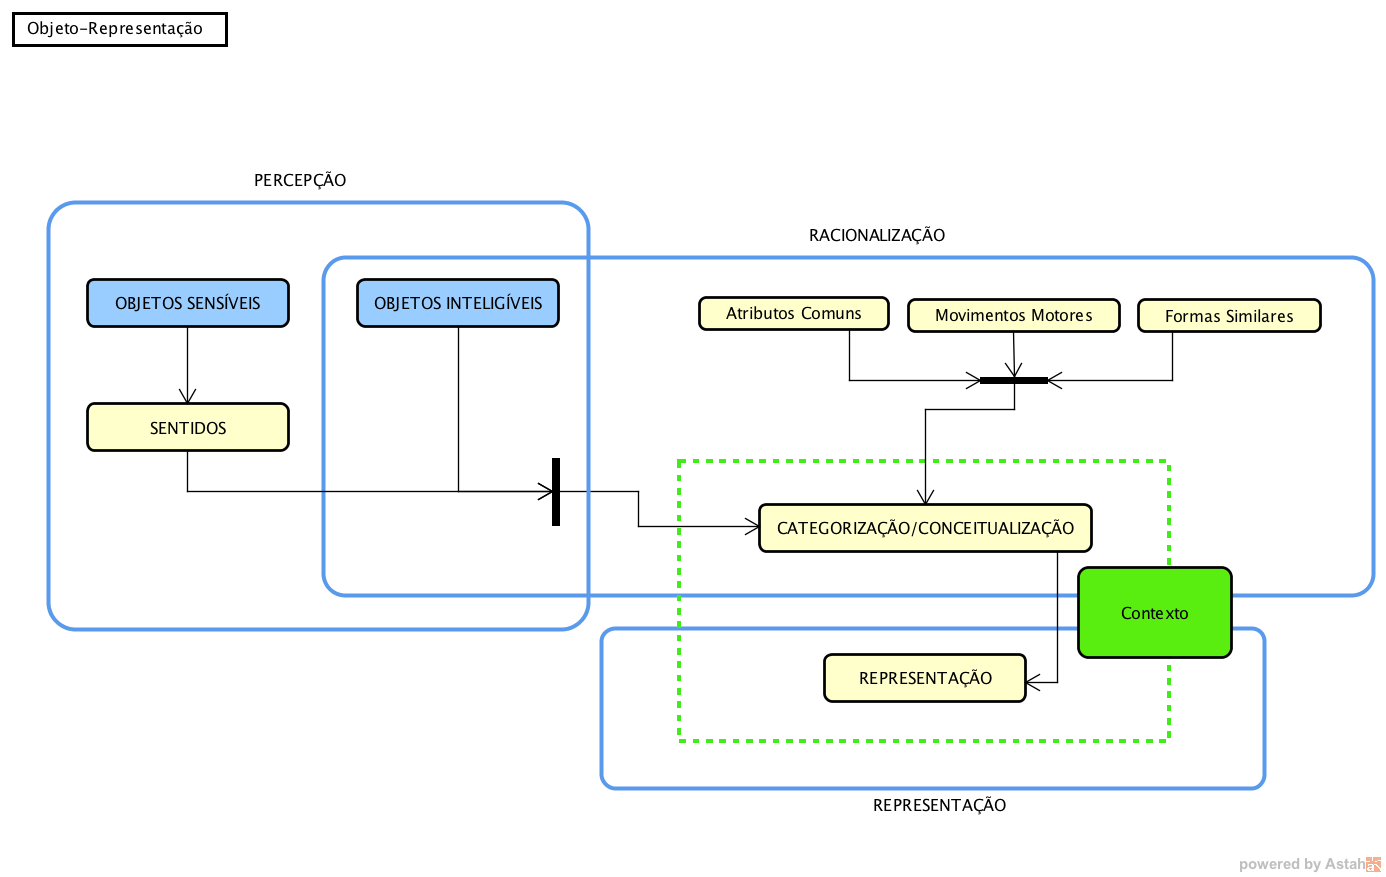
\includegraphics[angle=90, height=\textheight]{imagens/Fases_Processo_O-R.png}
    \caption{Fases do Processo Objeto-Representação}
    \label{fig:por-resumido}
\end{figure}

\section{\hspace*{3pt} Fase 01: Percepção}
\label{sec:percepcao}

A fase um foi definida como a Percepção, cuja função é fornececer os objetos que serão racionalizados. 

Objeto é tudo aquilo que nos circunda ou é designado pelo homem; são as ``coisas" do mundo. Nesta dissertação, o termo ``objeto” é empregado de maneira ampla e pode representar tanto objetos concretos (ex.: um animal ou um veículo), quanto objetos abstratos (ex.: um departamento ou um dragão) \cite{dahlberg:1978.teoria, machado:2009.projeto}. 

Podemos, ainda, categorizá-los em objetos sensíveis, isto é, aqueles objetos que são evidenciados para nós através de um, ou mais, sentidos e objetos inteligíveis, cuja sensação é fruto de um processo mental, como por exemplo a junção de ideias de mulher e peixe, para formar uma sereia ou conceitos que não existem de maneira física, como sentimentos. 

Ao categorizar os objetos em sensíveis e inteligíveis, apesar de reconhecer toda a batalha filosófica travada ao longo dos séculos entre as correntes denominadas Empirismo, Racionalismo e Criticismo, não estamos assumindo uma postura Empirista, mas queremos apenas evidenciar os objetos abstratos, como fruto um processo racional e reflexivo, a despeito de quaisquer discussões filosóficas subjacentes. 

A base da percepção humana são os sentidos, sendo estes estimulados de maneira contínua por um fluxo de acontecimentos. Disto resulta uma excitação neural chamada de sensação \cite{alexandre:2007.factores}.

Sensação, segundo o dicionário online \citeonline{priberam:2015} é ``a impressão produzida pelos objetos exteriores num órgão dos sentidos, transmitida ao cérebro pelos nervos, onde se converte em ideia, julgamento ou percepção''.

Na introdução da Crítica da Razão Pura, \citeonline{kant:1983.critica} afirma que: 

\begin{quote}
``Não há dúvida de que todo o nosso conhecimento começa com a experiência; do contrário, por meio do que a faculdade de conhecimento deveria ser despertada para o exercício senão através de objetos que toquem nossos sentidos e em parte produzem por si próprios representações, em parte põem em movimento a atividade do nosso entendimento para compará-las, conectá-las ou separá-las e, desse modo, assimilar a matéria bruta das impressões sensíveis a um conhecimento dos objetos que se chama experiência? […]" \cite[p.23]{kant:1983.critica}.
\end{quote}
 
Estas impressões, no entanto, são percepcionadas no espaço e no tempo, uma vez que formas puras (vazias) fazem parte das estruturas cognitivas inatas do sujeito. Elas são a condição indispensável para que possamos ter acesso ao conhecimento, isto é, a sensibilidade se expressa em duas formas: espaço e tempo, os  quais, nas palavras de \citeonline{kant:1983.critica}, são definidos, respectivamente, como:

\begin{quote}
``O espaço não é um conceito empírico abstraído de experiências externas. Pois a representação de espaço já tem que estar subjacente para certas sensações se referirem a algo fora de mim […] O espaço é uma representação a priori necessária que subjaz a todas as intuições externas. […] O espaço não é um conceito discursivo ou, como se diz, um conceito universal de relações das coisas em geral, mas sim uma intuição pura. […] O espaço é representado como uma magnitude infinita dada. […] A representação originária do espaço é, portanto, intuição a priori e não conceito" \cite[p.41]{kant:1983.critica}.
\end{quote}

\begin{quote}
``O tempo não é um conceito empírico abstraído de qualquer experiência. […] O tempo é uma representação necessária subjacente a todas intuições. […] Sobre essa necessidade a priori também se funda a possibilidade de princípios apodíticos das relações do tempo, ou de axiomas do tempo em geral. […] O tempo não é um conceito discursivo ou, como se diz, um conceito universal, mas uma forma pura da intuição sensível. […] A infinitude do tempo nada mais significa que toda magnitude determinada do tempo só é possível mediante limitações de um tempo uno subjacente" \cite[p.44--45]{kant:1983.critica}. 
\end{quote}

O espaço e o tempo não são conceitos, visto que não são elaborados pelo sujeito tendo como ponto de partida suas experiências; eles simplesmente existem no sujeito cognoscente, que ao conhecer os objetos do mundo, o fazem de um modo dimensionado e associado à ideia de movimento, de mudança, de evolução, ou mesmo em estágios ou locais diferentes. Por isso as noções de espaço e de tempo são condições necessárias para o conhecimento dos objetos do mundo.

É através de sua percepção que um indivíduo organiza e interpreta suas impressões sensoriais para atribuir significado ao seu meio. Do ponto de vista cognitivo, a percepção envolve processos mentais que interpretam os dados oriundos dos sentidos e os associam aos conceitos.

\section{\hspace*{3pt} Fase 02: Racionalização}
\label{sec:racionalizacao}

A racionalização quem nos permite dar significados aos estímulos que recebemos, transformando os dados oriundos das percepções em ideias ou conceitos.

Esta fase compartilha a visão atomística, que defende que a compreensão de um objeto implica o reconhecimento das partes para ter o entendimento do todo. Embora a visão holística - aquela que defende que a interpretação de um objeto se dá pelo todo - seja reconhecida, o todo quando inserido em um contexto, pode apresentar características que não sejam relevantes para a conceitualização do objeto.

Os experimentos propostos por \citeonline{rosch:1999.principles}, para encontrar o nível médio de abstração: atributos comuns, movimentos motores, forma objetiva e semelhança da forma, ou as forma de conhecer o mundo, quando dentro do contexto, permitem que identifiquemos quais características que são importantes para definição do objeto. 

O contexto delimita no universo do nosso discurso, qual as características dos objetos que percebemos fazem sentidos, e precisam ser compartilhadas para que nossas representações façam sentido para nossos interlocutores.  

A categorização reflete a nossa capacidade para agrupar entidades únicas em conjuntos, usando como regras de agrupamento as características que compartilham entre si. 

\subsection{\hspace*{3pt} Formas de Conhecer o Mundo}

Atributos comuns são as características que dois ou mais objetos de uma mesma categoria compartilham. Ex.: ter bicos, ter penas, por ovos.

Movimentos motores representam a maneira como interagimos determinados objetos, os movimentos musculares associados à utilização do objeto. Ex.: o ato de sentar em uma cadeira ou de cortar com um serrote.

Formas Objetivas e Similares dizem respeito a forma como o objeto se apresenta, isto é, a forma que ele possui. Ex.: cadeira de jantar, cadeira de praia, poltrona.

Nossa experiência associa características novas àquelas percebidas previamente, que sejam semelhantes. Refletir acerca da maneira como as características nos chegam nos ajudam entender como estamos categorizando um determinado grupo de características
            y
        
        %A noção de qualidade em modelos conceituais, o seu significado e como alcançá-la, ainda geram inúmeros debates por parte dos especialistas(Teeuw, WB; Van den Berg, H, 1997).

Pesquisas simplesmente listam propriedades desejáveis que podem ser encontradas em "boas" representações conceituais(Navathe, Shamkant B et al., 1992). Definições que são vagas e complicadas, e não existe qualquer estrutura subjacente que ajude a compreender as propriedades e como se relacionam umas com as outras. O resultado é um conjunto de avaliações ad hoc de representaçõeseconsenso sobre o que faz uma representação ser "boa"(Moody, Daniel L et al., 1998).

Segundo H James Nelson et al. (2012), diferentes frameworks tentam solucionar a problemática acerca da qualidade das representações de modelagens conceituais e das qualidades dos processos de modelagens conceituais. Destacamos oframework LSS introduzido por Odd Ivar Lindland et al. (1994)baseado na teoria semiótica de Morrise o framework desenvolvido por Yair Wand; Ron Weber, (1990)com base em teoria ontológica deBunge.

O framework sugerido porWand, Yair; Weber, Ron, (1990) é um processo atuante durante a modelagem, o que poderia interferir em nossas análises, por esse motivo optamos por utilizar a proposta de Odd Ivar Lindland et al. (1994), focada na análise do resultado do processo de modelagem. Em sua proposta três tipos de qualidade são introduzidos:

Qualidade Sintática: é o quanto um modelo conceitual e sua representação se correspondem. O conjunto de erros sintáticos contém todas as declarações que podem ser expressas no modelo, mas podenão ser feitana língua.
Qualidade Semântica: é o grau de correspondência entre o modelo conceitual e o mundo real. Se um modelo contém declarações que não têm correspondência no mundo real, o modelo é inválido, caso contrário, o modelo é incompleto.
Qualidade pragmática: é o grau de correspondência entre o modelo conceitual e sua interpretação (individual), ou seja, em até que grau um modelo é compreendido.

A qualidade sintática não será relevante neste trabalho, pois assumimos que os conceitos podem ser capturadas em uma linguagem adequada. E, a exemplo do que foi proposto em Teeuw, WB; Van den Berg, H, (1997) para capturar a qualidade semântica e qualidade pragmática, utilizaremos os seguintes critérios de qualidade:

Abrangência: Os conceitos devem ser expressivos o suficiente para capturar todos os "aspectos essenciais" do mundo real.
Clareza: Os conceitos e regras, bem como sua aplicabilidade, devem ser compreensíveis, sem dispêndio de muito tempo e esforço.
Consistência: Os conceitos não devem entrar em conflito uns com os outros nas representações dos aspectos do mundo real. Consistência implica não-ambiguidade: um conceito tem apenas um único sentido no mundo real.
Modularidade: aspectos independentes do mundo real devem ser capturados por diferentes conceitos, e aspectos fortemente relacionados devem ser representados por conceitos relacionados.
Os critérios apresentados abrangem a qualidade "externa" dos conceitos, àquelas utilizadas para a satisfação dos usuários, e a qualidade "interna", as propriedades intrínsecas dos conceitos.

5.1. Metodologia

Procuramos avaliar se a utilização do processo proposto neste trabalho, e suas teorias subjacentes, promovem uma melhoria nos modelagem conceitual e, por conseguinte, em sua representação correspondente.

Castro, Lúcia, (2010) aponta as dificuldades existentes para a mensuração de propriedades qualitativas em modelos conceituais, e explica que, tal análise demanda a aplicação das teorias e técnicas propostas em uma situação real, ou em um estudo de caso.

5.1.1. O Estudo de Caso

Para o estudo de caso apresentado, optamos por uma abordagem pictográfica para a apresentação do contexto.Souza, Tania, (1998) argumenta que a referencialidade sustenta a possibilidade de leitura da imagem e, por outro lado, reafirma o seu status de linguagem.

A descrição textual, conformeHeuser, Carlos Alberto, (2001) e Machado, Felipe Nery Rodrigues; Abreu, Maurício Pereira de, (2009), fornece importantes dicas acerca de quais objetos, relações e atributos são relevantes para o contexto. Trabalhos como o deCastro, Lúcia, (2010) e Leão, Felipe et al. (2012), apresentam abordagens para a modelagem conceitual pautada em descrições textuais. Neste sentido as imagens tentaram favorecer a explanação do contexto e de suas atividades, deixando os participantes livres para a interpretação do contexto sem, no entanto, transmitir quaisquer informações explícitas.

Para participar desta fase da pesquisa, foram convidados analistas de sistemas, com conhecimentos na área de desenvolvimento de software, especificação de software ou Bancos de Dados.

Com o objetivo de avaliar a aplicação do POR, dividimos os participantes em dois grupos, o grupo A e o grupo B, e em cada grupo realizamos duas rodadas de modelagens, com o intuito de responder a questões distintas.

No grupo A, estávamos interessados em avaliar se o POR influenciaria a descoberta de conceitos pertinentes a um determinado contexto, e se essa representação seria mais completa.

No grupo B, nosso intuito era analisar se, uma vez apresentados ao processo, os modeladores utilizaram as fases descritas para a elaboração de novos modelos, mesmo quando não solicitado que o utilizassem.

Na primeira rodada, para cada participante, em ambos os grupos, uma série de imagens foram apresentadas, cada imagem continha uma cena peculiar, que apresentava o contexto de uma livraria e em algumas delas, havia a sugestão da realização da compra de livros.

Após essa exposição, cada participante foi instruído a elaborar um modelo conceitual, utilizando a linguagem de sua preferência para a representação deste contexto. O modelo deveria expor o contexto, com toda riqueza de detalhes (conceitos, características e relações) que o participante julgasse necessária para expressá-lo, em especial sua atividade fim, sem ambiguidades.

O grupo A deveria executar essa modelagem sem o auxílio do processo OR, ao passo que o grupo B foi apresentado ao processo proposto neste trabalho, e deveria efetuar sua elaboração considerando as fases de aquisição, categorização e representação dos conceitos percebidos.

Na segunda rodada, o grupo A foi apresentado ao processo, e lhes foi solicitado que considerando o exposto, revisassem o modelo criado previamente, refazendo-o caso julgassem necessário.

Enquanto que ao grupo B, um novo contexto com uma tarefa específica, desta vez com imagens mais explícitas, foi apresentado e solicitado um modelo que fosse capaz de representá-lo.

Para efetuar a captura de dados, o processo de modelagem foi gravado, e as gravações analisadas.

5.1.2. Avaliação dos Processos e Modelos

Esta avaliação propõe-se a entender como os participantes entendem o contexto e que conceitos são capazes de alcançar através da observação das imagens e reflexão sobre o contexto e suas atividades.

5.1.2.1. Grupo A

O primeiro participante do grupo A, que chamaremos de A1, é analista de sistemas e possui 10 anos de experiência, tendo trabalhado para empresas do setor público e privado, desenvolvendoatualmentepara uma instituição federal, atuando principalmente na área de análise e modelagem de requisitos.

Em sua modelagem, o analista A1, observou que o contexto tratava-se de uma livraria e seu primeiro conceito destacado no modelo foi o de livro. Porém no decorrer na elaboração, deu-se conta de que o conceito livro, era um termo com intensão note muito específica, e que embora trouxesse clareza para seu modelo, sua abrangência era muito limitada, o que o fez optar por outro conceito, o de publicação, e associou ao conceito de tipo de publicação. O tipo de publicação, a fim de trazer consistência e modularidade, demandaria a especificação dos tipos de publicação, no entanto o analista A1 não o fez, deixando-o subjetivo.

O analista A1 também entendeu que toda publicação estava localizada em uma seção e também deveria ter um autor, e ocasionalmente seria comprada por um cliente. O conceito cliente se evidenciou com mais facilidade, porém ao retornar às imagens que descreviam o contexto, o analista sentiu necessidade de representar o conceito compra e escolheu o símbolo adquire para nomeá-lo em um primeiro momento, alterando-o para compra pouco tempo depois. Aqui novamente pode-se perceber a escolha por um conceito que transmitisse maior clareza e abrangência. Clareza porque adquirir não deixa claro como se deu a aquisição e abrangência porque compra, evidencia o aspecto essencial da atividade fim de uma livraria.

Finalizou seu modelo, detectando a necessidade de acrescentar o conceito tipo de pagamento em relação acompra, a fim de melhorar a modularidade do conceito de compra.

Nenhum outro conceito foi apresentado ou quaisquer características listadas, embora se possa perceber, através das suas escolhas acerca de quais símbolos utilizar para representar os conceitos e que características distintas foram levadas em consideração, por exemplo para a troca do conceito livro por publicação ou o conceito aquisição por compra.

A Figura 11 demonstra o resultado final do modelo do analista A1, após a primeira rodada.


Modelo gerado pelo analista A1 sem o POR
Após a apresentação do POR, o analista A1 foi convidado a rever sua modelagem, no entanto, sentiu necessidade de efetuar poucas mudanças na distribuição dos conceitos, adicionando apenas o conceito editora.

Porém, sua nova análise apontou a necessidade de elencar características que definem cada conceito. Podemos perceber em seu novo modelo, Figura 12, que algumas dessas características foram adicionadas como atributos seguindo o paradigma da linguagem UML e outros como comentários. 

Outra aspecto alterado foi a descrição dos papeis executados por cada conceito, favorecendo a clareza desses conceitos. Algumas características, como as representadas pelos símbolos livro e revista, apesar de explicitados não se tornaram novos conceitos no modelo, algo que poderia favorecer a consistência e a modularidade do modelo final.


Modelo gerado pelo analista A1 com o POR
O segundo participante do grupo A, que chamaremos de A2, possui formação e experiência acadêmica apenas, sem quaisquer experiências no mercado de trabalho.

O analista A2 iniciou sua modelagem através do conceito item, e representou explicitamente suas características. Em seguida definiu os conceitos livro e revista como conceitos de menor abrangência em relação ao conceito item. Segundo a linguagem UML, escolhida para representar o contexto, essa configuração caracteriza uma herança. O analista continuou, apontando as características dessas heranças e relacionou o conceito pai, item, ao conceito pedido através de uma relação.

O símbolo item embora possua uma grande abrangência, sozinho, não traz ao modelo clareza, consistência ou modularidade, mas ao ser definido como um conceito pai, de livro ou revista, não só resolve esses problemas, como também demonstra que para o analista A2 ambos os conceitos são tipos de itens, isto é, evidencia sua categorização racional.

O analista também identificou na sequência o conceito item estoque; pedido do cliente, cliente, pedido fornecedor. Declarando as relações de herança de pedido cliente e pedido fornecedor ao conceito pedido; e uma relação direta entre item estoque e item; e outra relação direta entre cliente e pedido cliente. Identificou o conceito vendedor e declarou uma herança, considerando cliente e vendedor, como filhos em relação ao conceito pessoa física. Pessoa jurídica, após ser declarada, foi adicionada como um conceito filho, junto com pessoa física ao conceito pessoa.

Podemos perceber que determinados conceitos, demandam outros conceitos. Como percebido na modelagem do analista A2, onde compra é feita por cliente, que efetua um pedido, que possui item de pedido, que é retirado do estoque.

Da mesma maneira aqui, a compra gera baixa no estoque, que precisa ser reposto por um fornecedor, através de um pedido de compra onde constam itens para a reposição.

Pessoa jurídica deu origem a um conceito filho, denominado fornecedor. E este colocado em relação direta com conceito pedido fornecedor. Todas as características, de cada um dos conceitos, foram listadas, o que indica o favorecimento de uma melhor descrição do contexto.

A análise do contexto efetuada pelo analista A2 revelou conceitos que não estavam implícitos nas imagens, como fornecedor, estoque, mas que foram evidenciadas ao considerar os conceitos presentes no contexto. Seu modelo, está representado pela Figura 13.


Modelo gerado pelo analista A2 sem o POR
Após ser apresentado ao POR, o analista foi convidado a rever sua modelagem. O analista apresentou certa confusão ao repensar o domínio, e não parecia estar muito certo sobre como proceder na passagem pelo processo. Confusão que foi sanada após alguns questionamentos acerca das etapas, e apresentação de alguns exemplos. No final deste, o analista optou por refazer o modelo utilizando metamodelo Entidade-Relacionamento.

Com esta abordagem, o analista utilizou-se da marcação de relacionamento típico do metamodelo E-R, o losango, para representar relações que julgava necessárias.

Nesta nova abordagem, o analista começou sua apresentação através do conceito livro, para o qual foram definidas as mesmas características listadas no modelo anterior. Porém percebemos que a utilização do processo OR, o levou a analisar quais outras características são essenciais para o conceito livro, dentro do contexto livraria, fazendo com que fosse representado a relação de pertencimento a uma coleção. Além de outras características definidoras do mesmo, em uma relação de posse, a citar: número de páginas, tipo de página, capítulos, imagens, orelha, capa, contracapa, categoria. Todas após definir a relação de posse.

Embora essas características não tenha sido representadas dentro do conceito livro, como atributos, fica evidente que as características adicionam clareza e modularidade ao conceito.

Para o conceito revista, segundo a ser representado, a exemplo do livro, o analista atribuiu as mesmas características do primeiro modelo.

A Adição da última característica, índice, no conceito revista o fez retornar ao conceito livro e também adicionar índice e subtítulo como características.

Após suas representações, o analista generalizou os conceitos, adicionando ambos como filhos do conceito item, e nomeando os papéis. Transformando a abordagem anterior top-down, em uma abordagem bottom-up, isto é, definindo primeiro os conceitos de menor abrangência e a partir deles, os conceitos de maior abrangência.

A partir deste ponto, o analista apenas replicou o modelo anterior, porém acrescentando as relações entre os conceitos e nomeando os papeis, como podemos verificar na Figura 14.


Modelo gerado pelo analista A2 com o POR
5.1.2.2. Grupo B

No grupo B, o primeiro analista, aqui chamado de analista B1, declarou possuir 10 anos de experiência na área de TI e que mais da metade de suas atividades possuem relação ou estão diretamente ligadas à modelagem conceitual.

Após ser apresentado ao processo OR, o analista B1 iniciou sua tarefa de modelagem e identificou sem maiores problemas o contexto que deveria representar.

Sua representação iniciou-se pelo conceito livro, e foi seguido pelos conceitos que representavam a atividade fim do contexto, isto é, a venda de livros. Em sua representação, o analista B1 adicionou as características que julgou mais importantes a todos os conceitos, e através dos construtos da UML, representou as relações de composição e agregação existentes entre os conceitos identificados, isto é, as relações parte-todo.

Somente após essa representação mais imediata da atividade fim do contexto, o analista expandiu sua representação, porém trazendo mais elementos que compunham a atividade de venda. Nesta expansão, uma herança foi adicionada, na forma do conceito mais geral, representado pelo símbolo pessoa e três conceitos mais individuais, representados pelo símbolos vendedor, autor e cliente.

Apesar de utilizar o POR, o analista não distinguiu de maneira clara os tipos de publicações existentes nas imagens e nem considerou a reposição do estoque, embora tenha declarado a existência da característica que remeteria a este conceito. Escolha que, considerando os critérios de qualidade utilizados, não favorece o modelo quanto à modularidade e abrangência. A definição de um conceito categoria, com a característica de nome, não favorece a clareza. 

Uma conclusão possível seria que o analista optou por uma abordagem direta, focada na atividade fim do contexto, representando apenas os conceito imediatos, dentre os quais, apesar de haver revistas nas prateleiras, não havia imagem que mostrasse a compra de uma revista.

Fato que pode reforçar essa análise é a representação dos conceitos autor, editora e categoria, relacionados com o conceito livro. Conceito que estava imediatamente representado nas imagens de prateleiras e de compras.

Outro ponto a se destacar é o fato de que, para os conceitos representados, o analista atribuiu características que, segundo sua análise, eram essências para a definição destes mesmos conceitos.


Modelo gerado pelo analista B1 com o POR
Assim que o analista declarou o fim de seu modelo, foi lhe solicitado querealizasse uma nova tarefa de modelagem. Porém sem a utilização do processo apresentado neste trabalho.

O novo contexto representava a aquisição de ingressopara um espetáculo teatral. Contexto que foi interpretado de imediato pelo analista B1, e seu conceito primáriofoi exatamente o de um espetáculo.

Em sua representação, o analista B1 foi capaz de destacar conceitos como personagem, artista, produtor executivo e patrocínio, conceitos que não eram sugeridos através das imagens e que, apesar de se relacionarem com o contexto, não remetiam à tarefa de comprar de ingresso.

A representação dos conceitos pode indicar a permanência, de maneira subjetiva, das faixas que compunham o POR, em especial a fase 2, que diz respeito a racionalização. Suspeita estasustentada pela existência de conceitos que na verdade poderiam ser alcançados definindo as características essenciais de um espetáculo.

Quando sua representação é analisada sob os critérios de qualidade designados, apenas se considerarmos os tipos de espetáculos que podem estar em cartaz em um teatro, o critério de modularidade não é atendido. No entanto, a representação possui clareza, abrangência e consistência.


Modelo gerado pelo analista B1 sem o POR
O analista B2possui experiência de dez anos na área de desenvolvimento de softwarese tem experiência com bancos de dados. Optou, para sua representação, pela descrição textual e, em sua elaboração do modelo, começou sua representação através do conceito livro. Destaca-se o fato de que, ao descrever as características do conceito livro, declarou o tempo de entrega.

Sua abordagem seguiu a conexão de conceitos esperada, isto é, uma compra, tem itens e esses itens precisam ser pagos. Seu modelo reflete esse pensamento ao definir os conceitos pedido, item do pedido e pagamento.

Para cada conceito, o analista B2 listou cada uma de suas características, declarando aquelas que efetivamente uniam um conceito aoutro. Durante sua modelagem, pôde-se observar alguns minutos onde parecia analisar o próximo conceito a ser inserido e se as características listadasrepresentavam bem o conceito já representado.

Este analista também, embora defina uma característica quantidade em estoque, não representa a possibilidade da existência de um fornecedor, assim como não considera a existência de outros tiposde publicações nas imagens que definem o contexto.

Podemos perceber que, apesar de nenhuma imagem fazer alusão a comprason-line, o analista B2 considerou sua representação para um ambiente web. Essa análise é motivada pela existência do conceito endereço e pela característica tempo de entrega, atribuída ao conceito livro.

O que nos leva a crer que, também em busca de uma objetividade, o analista apenas considerou a atividade fim do contexto.

Sua representação textual encontra-se logo abaixo:

Livro
isbn
titulo
descrição
quantidadeEstoque
preçoVenda
tempoEntrega
categoria (Referência para classe categoria)
Categoria
id
nome
descrição
Cliente
cpf
nome
endereço (Referência para classe endereço)
telefone
email
Endereço
rua
cep
bairro
numero
cidade
estado
país
complemento
Pedido
numero
data
endereçoEntrega (Referência para classe endereço)
status
cliente (Referência para classe cliente)
Pagamento
numero
valor
data
pedido (Referência para a classe Pedido)
lista de item do pedido (Referência para classe itemPedido)
itemPedido
livro (Referência para classe livro)
quantidade
Após a finalização da elaboração do modelo, o novo contexto lhe foi apresentado e sua representação iniciou-se com o conceito espetáculo. O analista apontou seis conceitos explicitamente e cada uma das características que julgou necessária, incluindo as relações que teriam.No entanto, comentou que conceitos como funcionário ou categoria de espetáculos poderiam ser representados, mas não sentiu necessidade de explicitá-las visto que sua representaçãoapresentava minimamente o conceito. 

Considerando a tarefa específica de compra de ingresso, a representação do analista atende aos critérios de qualidade listados.

Espetáculo
id
nome
tempo de duração
Cliente
id
nome
endereço (Ref. para classe endereço)
Endereço
rua
cep
bairro
....
Sala
id
nome
Sessão
sala (Ref. para classe sala)
espetáculo (Ref. para classe espetáculo)
data/hora início
data/hora fim
preço
número de assentos disponíveis
Compra
sessão (Ref. para classe sessão)
cliente (Ref. para classe cliente)
forma de pagamento
assento comprado
Podemos observar, para ambos os analistas do Grupo B, que a escolha do conceito de maior abrangência, em detrimento de uma maior especificação - como por exemplo o conceito apresentação, visto que a imagem destacava um grupo de balé - pode ser reflexo do entendimento de que uma peça de teatro e um concerto também representam um espetáculo. Evidenciando uma escolha por um conceito mais geral para tornar o modelo mais genérico. De encontro com essa observação, podemos ressaltar o fato de que o analista B1 entende que espetáculos são compostos por atores e personagens.

O analista B1 relatou após a elaboração do modelo conceitual, de maneira informal, que ao utilizar o processo Objeto-Representação percebeu que muitas de suas assunções, feitas de maneira automática, foram reconhecidas no processo e que o mesmo ajuda a focar nos conceitos importantes, sem se aprofundar em demasia ou em escassez, o que pode significar um ganho de tempo na busca da melhor maneira de representar um conceito.

O analista B2reiterou, após a execução da tarefa, que regras não estavam explícitas em seu modelo, tais como verificar se haveria assento disponível antes de efetuar a venda.



Neste capítulo foi apresentadaa metodologia para avaliação da proposta deste trabalho, a fim de averiguar se o Processo Objeto-Representação era capaz de guiar os modeladores através dos conceitos e de suas concepções. Nosso objetivo principal foi comparar os resultados dos modelos criados pelos analistas sem a aplicação do método, com os modelos resultantes com sua aplicação, a fim de perceber a definição de conceitos e características que antes não haviam sido representados em uma análise qualitativa.

Observamos que a descoberta de novos conceitos foi possível, mas apesar disto, nem todos passaram a figurar exatamente como conceitos nos modelos. Alguns foram listados como características de conceitos já existentes.

Da mesma forma, buscou-se observar se após o contato com o processo, haveria a continuidade da reflexão acerca da formação dos conceitos, em busca da melhor representação do mesmo. A conclusão desta avaliação, embora não possa ser percebida de maneira explícita nos modelos resultantes, pode ser observada, na escolha proposital de conceitos mais gerais para representar o contexto, diante de uma tarefa específica.

Finalmente,a avaliação aqui propostasugere que a adoção de um processo que explicita o reconhecimento do objeto e os caminhos percorridos por nosso intelecto até sua representação, podem ajudar modeladores a pensarem os contextos que estão tentando representar, levando-os a considerarem conceitos e características até então não haviam sido considerados. A avaliação sugere também, que o processo, ao analisar um dado conceito inserido no seu contexto, pode auxiliar o modelador na escolha do símbolo para representar este conceito, no modelo conceitual que está sendo elaborado.
        %Este trabalho teve como foco a qualidade semântica e a qualidade pragmática de um modelo conceitual. Foi defendido que, para um modelo alcançar esses objetivos, o correto entendimento acerca das características que definem cada conceito, assim como suas relações, precisam ser entendidas e pensadas de maneira adequada. Para isso, é preciso reconhecer o objeto da reflexão, entender os processos que permitem apreender o objeto, contextualizar esse objeto, apontar quais as características deste objeto são relevantes neste contexto, buscar suas relações com outros objetos deste contexto, para então definir o símbolo que o representará.

Como apoio teórico, esse trabalho propõe um processo baseado nas teorias da filosofia, da psicologia e na linguística. A interseção destas três áreaspermitiu a reflexão na busca pelo processo de racionalização dos conceitos.

Outros trabalhos realizados na área da Ciência da Informação,atestam a significância e relevância das áreas utilizadas, seja individualmente ou em conjunto. Abaixo destacamos alguns trabalhos relevantes para nosso estudo e suas principais distinções da nossa abordagem.

Maria Luiza de Almeida Campos, (2001)apresenta uma metodologia de criação de hipertextos, onde os conceitos envolvidos na determinação de relacionamentos entre links devem ser considerados. Seu método está dividido em três níveis de entendimento e compreende sete requisitos básicos, onde questões como domínio do conhecimento, leitor final, identificação de conceitos e relacionamentos entre os nós, estabelecimento do veículo de comunicação são discutidas. O Processo Objeto-Representação embora esteja dividido em três fases, concentra-se na identificação das características que definem um determinado conceito no âmago do modelador e busca guiá-lo para que a representação desse conceito conserve todas as características e relacionamentos observados.

Em Bernardo Pereira Nunes et al. (2009), é apresentado uma técnica para classificação hierárquica automática de dados semiestruturados. Baseado na teoria de protótipo o trabalho buscou organizar os frames, através de seus atributos definidos como principais, em uma hierarquia. No Processo Objeto-Representação buscamos entender porque determinados atributos são tidos como principais em um dado contexto.

Rafael dos Santos Nonato; Gercina Ângela Borém de Oliveira Lima, (2012), buscou os aspectos importantes no tratamento da informação e da determinação de links em hipertextos. Em seu trabalho utilizando o protótipo MHTX, buscou em uma estrutura de navegação dividida em facetas encontrar novos relacionamentos para os links utilizando glossários e dicionários gerais. O Processo Objeto-Representação, neste aspecto busca os relacionamentos que um objeto possa ter com outros no próprio modelador e sua experiência com o contexto analisado, na busca da representação que permita o entendimento do conceito pelo maior numero de pessoas possíveis.

Naziozenio Antonio Lacerda, (2012)em seu trabalho mostrou-se interessado em entender qual seria a concepção dos educadores sobre tecnologia digital, buscando fundamentos que pudessem trazer novas perspectivas ao processo. No entanto, manteve-se focado na descrição de um único conceito. O Processo Objeto-Representação busca uma orientação que possa servir de base para auxiliar a descrição de contextos diversos.

Embora cada uma das áreas tenhacontribuições significativas, os trabalhos vistos não apresentaram um processo que abarcasse as três grandes áreas. Os resultados das avaliações indicam que a abordagem através do processo pode orientar os modeladores na descoberta do conceito mais adequado para expressar um objeto inserido em um contexto, originando um modelo conceitual semântico e pragmático.

6.1. Principais Contribuições

A principal contribuição deste trabalho é a apresentação de um processo para orientar a descoberta de conceitos em modelo conceitual. Esse processo, com aporte nas teorias da Filosofia, Psicologia e Linguística é estruturado em três fases, onde o resultado das reflexões de cada faseé o insumo para a fase seguinte.

Entendendo que a modelagem conceitual é uma área importante para a correta apreensão de conhecimento acerca de um domínio, o seu entendimento e sua representação fidedigna. Consideramos como boas práticas que poderiam auxiliar a utilização do Processo Objeto-Representação, em um primeiro momento a correta limitação do contexto acerca do qual se pretende emitir enunciados. Essa limitação, embora seja apresentada na Fase 02 seguindo o fluxo racional, trará maiores benefícios para os modeladores se forem observadas desde o primeiro momento, pois assim poderá definir quais conjuntos de palavras fazem mais sentido dentro do contexto em questão.

Afim de facilitar o processo de modelagem devemos, em um segundo momento, definir as maneiras através das quais interagimos com os objetos, isto é, quais são as formas de conhecer o mundo. Esse processo pode ser percebido ao nos depararmos com um objeto e buscarmos em nossa experiência objetos que possuam características semelhantes, objetos com quais interagimos ou utilizamos da mesma maneira, ou ainda objetos que apresentem forma final ou útil próxima. Esse entendimento nos levará naturalmente a enunciar cada uma das características que pudermos perceber no objeto, fornecendo uma lista que nos permitirá analisar quais destas características são necessárias para esse objeto seja relevante no contexto definido.

O processo de definição das características necessárias, envolve perceber como essas características se relacionam umas com as outras e, posteriormente, como o objeto como um todo se relaciona com outros objetos presentes no mesmo espaço contextual definido. Essa percepção permitirá encontrar a representação que, dentro do contexto, permitirá a transmissão mais adequada do conceito.

Essas recomendações geraispodem ser melhor visualizadas abaixo:

Delimitar o contexto no qual os objetos estão inseridos e através do qual serão representados.
Observar de maneira ampla os objetos que compõe o contexto, sem se preocupar com as representações que possam expressar os objetos apreendidos.
Distinguir de maneira clara quais sensações são despertadas pelo objeto, isto é, que sentidos são responsáveis pela apreensão do mesmo, ou se o objeto é um objeto inteligível.
Entender as maneiras pelas quais podemos conhecer esses objetos, descrevendo em enunciados curtos essas maneiras.
Organizar essas as características enunciadas de maneira a evidenciar suas relações umas com as outras e dos objetos entre si.
A utilização do processo permite:

A identificação de conceitos que de outra maneira poderiam ser identificados tardiamente.
A escolha adequada do símbolo para representar o conceito, trazendo clareza, consistência e codularidade para o modelo conceitual resultante.
Uma sistematização do processo de racionalização de um conceito, evidenciando o conhecimento acerca do objeto e sua aquisição.
A utilização do processo permite que linguagens distintas, utilizadas para a representação de contextos reais, sejam beneficiadas, poiso foco principal do processo está na escolha adequada dos conceitos e, o mais importante, em como saber que tal conceito é o mais indicado para evocar uma ideia. Tal propósito permite que sua utilização traga proveito para as linguagens de modelagens mais distintas, desde as mais simples como a Entidade-Relacionamento, até as mais expressivas.

6.2. Trabalhos Futuros

Para trabalhos futuros pretendemos analisar como as áreas da Antropologia, Inteligência Artificial e Neurociência se relacionam com as áreas exploradas neste trabalho, de acordo com o hexágono cognitivo apresentado em Gercina Ângela Borém Lima, (2003). Realizar mais experimentos utilizando um universo mais amplo, buscando modeladores com diferentes níveis de conhecimento, com o objetivo de ampliar os estudos sobre o processo e sua utilização.Será preciso analisar, sob o prisma das modelagens com aporte ontológicos,como a proposta porGiancarlo Guizzardi, (2005), se nosso processo é capaz de fornecer algum ganho aos modeladores e a esses processos. Pretendemos verificar se o Processo Objeto-Representação poderia apresentar ganho na modelagem realizada por grupos de modeladores, tanto de uma mesma área de conhecimento, como de áreas de conhecimentos distintas.

Aplicar o Processo Objeto-Representação em contexto diferente da modelagem conceitual, como o de buscas web por exemplo. Uma outra abordagem seria a criação ou adaptação de uma ferramenta que dê suporte as fases do processo.Outra possibilidade seria a utilização de mais abordagens teóricas acerca da aquisição,classificação, categorização e representação do conhecimento, afim de prover melhor aporte aos modeladores   
        
 \addcontentsline{toc}{chapter}{Referencias}

\bibliography{postexto/referencias}

\end{document}